% =====================================================================
%  Aperio: The Complete Guide
%
%  A single-file LaTeX book covering the whole system: architecture,
%  configuration, routing, security, operations and reference tables.
%
%  Build (any of):
%      pdflatex aperio.tex && pdflatex aperio.tex   % twice, for the TOC
%      latexmk -pdf aperio.tex
%      tectonic aperio.tex
%
%  Packages come from a normal TeX Live / MacTeX installation (tcolorbox
%  and pgf/TikZ included, so a *minimal* install is not enough); nothing
%  is downloaded at build time beyond what those distributions ship.
%  `tectonic aperio.tex` fetches what it needs on first run.
%
%  Conventions used throughout:
%    - \code{}  inline literal (command, key, header, identifier)
%    - server / client blocks always name which side they run on
%    - every setting is shown in its yaml form first, env in a comment
% =====================================================================
\documentclass[11pt,a4paper,oneside]{book}

\usepackage[T1]{fontenc}
\usepackage[utf8]{inputenc}
\usepackage{lmodern}
\usepackage[margin=2.6cm, headheight=14pt]{geometry}
\usepackage{microtype}
\usepackage{xcolor}
\usepackage{booktabs}
\usepackage{longtable}
\usepackage{array}
\usepackage{enumitem}
\usepackage{fancyhdr}
\usepackage{listings}
\usepackage{titlesec}
\usepackage{tikz}
\usetikzlibrary{arrows.meta, positioning, shadows}
\usepackage{graphicx}
% Both spellings, so the book builds from its own directory and from the
% repository root (`tectonic docs/book/aperio.tex`) alike.
\graphicspath{{../images/}{docs/images/}}
\usepackage{colortbl}
\usepackage{tcolorbox}
\tcbuselibrary{listings, skins, breakable}
\usepackage[hidelinks]{hyperref}

% --- Colours -------------------------------------------------------
% The accent is the product's own: the dashboard's primary is
% oklch(0.532 0.157 131.589), which is this green. A book that looks like
% the thing it documents is doing part of the explaining for free.
% The mark's own green (docs/assets/aperio-mark.svg). It is a signature
% colour, not a text colour: at 12pt on white it does not carry, so it is
% used for rules, frames and labels, and never for a paragraph.
\definecolor{AperioGreen}{HTML}{00A85C}
\definecolor{TableRule}{HTML}{D6DBE0}
\definecolor{AperioGreenLight}{HTML}{F2F8EA}
\definecolor{CodeBg}{HTML}{F8F9FA}
\definecolor{CodeFrame}{HTML}{CBD5E1}
\definecolor{CodeHeaderBg}{HTML}{E9EEF3}
\definecolor{CodeComment}{HTML}{6A737D}
\definecolor{CodeString}{HTML}{032F62}
\definecolor{CodeKey}{HTML}{005CC5}
\definecolor{TextDark}{HTML}{212529}
\definecolor{RuleGrey}{HTML}{BBBBBB}

% --- Headings -------------------------------------------------------
% Sans-serif and accented, against the serif body: a heading should be
% findable while flicking through eighty pages of prose.
% The chapter title is set in the body's dark, not in the accent: eight
% words of saturated green at 24pt is a colour swatch, not a heading. The
% accent goes on the label above it, which is what tells you where you are.
\titleformat{\chapter}[display]
  {\normalfont\sffamily\huge\bfseries\color{TextDark}}
  {\sffamily\large\bfseries\color{AperioGreen}\chaptertitlename\ \thechapter}{10pt}{\Huge}
\titleformat{\section}
  {\normalfont\sffamily\Large\bfseries\color{TextDark}}
  {\thesection}{1em}{}
\titleformat{\subsection}
  {\normalfont\sffamily\large\bfseries\color{TextDark}}
  {\thesubsection}{1em}{}

% --- Inline literals ------------------------------------------------
% Every literal goes through \code so the styling is uniform. Underscores
% inside the argument are escaped at the call site (\_), which keeps this
% macro usable in section titles and table cells where \verb is not.
\newcommand{\code}[1]{\texttt{\small #1}}

% --- Code listings --------------------------------------------------
\lstdefinestyle{aperio}{
  basicstyle=\ttfamily\footnotesize,
  commentstyle=\color{CodeComment}\itshape,
  stringstyle=\color{CodeString},
  keywordstyle=\color{CodeKey}\bfseries,
  breaklines=true,
  breakatwhitespace=false,
  columns=fullflexible,
  keepspaces=true,
  showstringspaces=false,
  frame=leftline,
  framesep=6pt,
  rulecolor=\color{RuleGrey},
  xleftmargin=10pt,
  aboveskip=10pt,
  belowskip=10pt,
  captionpos=b,
}
\lstset{style=aperio}

\lstdefinelanguage{aperioyaml}{
  morecomment=[l]{\#},
  morestring=[b]",
  morekeywords={true,false,null},
  sensitive=true,
}
\lstdefinelanguage{aperiosh}{
  morecomment=[l]{\#},
  morestring=[b]",
  morekeywords={curl,docker,aperio-client,aperio-server,export,printf,jq,check},
  sensitive=true,
}
\lstdefinelanguage{aperiojson}{
  morestring=[b]",
  morekeywords={true,false,null},
  sensitive=true,
}

% --- Code cards -----------------------------------------------------
% A titled box around a listing. The title carries the one thing a reader
% has to know before reading a line of it: which side it runs on, or
% which file it belongs in. The book's convention used to put that in a
% comment on the first line, where it competed with the code.
\newtcblisting{codecard}[2][aperiosh]{
  enhanced,
  breakable,
  arc=4pt,
  boxrule=0.8pt,
  colframe=CodeFrame,
  colback=CodeBg,
  coltitle=TextDark,
  fonttitle=\sffamily\bfseries\small,
  colbacktitle=CodeHeaderBg,
  title={#2},
  attach boxed title to top left={xshift=10pt, yshift=-10pt},
  boxed title style={arc=3pt, boxrule=0.5pt, colframe=CodeFrame,
                     colback=CodeHeaderBg, boxsep=2pt, left=6pt, right=6pt},
  top=14pt, bottom=8pt, left=8pt, right=8pt,
  listing only,
  listing options={style=aperio, language=#1, frame=none, xleftmargin=0pt,
                   aboveskip=0pt, belowskip=0pt}
}

% --- Headers --------------------------------------------------------
\pagestyle{fancy}
\fancyhf{}
\fancyhead[L]{\small\sffamily\nouppercase{\leftmark}}
\fancyhead[R]{\small\sffamily\thepage}
\renewcommand{\headrulewidth}{0.4pt}

% --- Admonitions ----------------------------------------------------
% Same interface as before (\begin{aperionote}{Title}), a box rather than
% a pair of rules: a callout that is skimmed past is a callout wasted.
\newtcolorbox{aperionote}[1]{
  enhanced,
  breakable,
  colback=AperioGreenLight,
  colframe=AperioGreen,
  arc=4pt,
  boxrule=0.8pt,
  leftrule=4pt,
  % The title sits inside the box rather than in a bar of its own: a
  % coloured bar the width of the page reads as a section, and these are
  % asides. `colbacktitle` matches the body so it is one block.
  title={#1},
  coltitle=AperioGreen,
  colbacktitle=AperioGreenLight,
  fonttitle=\sffamily\bfseries,
  attach title to upper=\par\medskip,
  top=8pt, bottom=8pt, left=10pt, right=10pt
}

\newcommand{\aperiokey}[1]{\subsubsection*{\code{#1}}}

% --- Reference table rows -------------------------------------------
% Entries in the appendices are paragraphs, several lines each, and with
% nothing but vertical space between them the eye cannot tell where one
% ends and the next begins. A hairline can: light enough to stay out of
% the way, dark enough to find.
\newcommand{\rowsep}{%
  \arrayrulecolor{TableRule}\specialrule{0.4pt}{2.5pt}{2.5pt}\arrayrulecolor{black}}

% --- Diagram styles -------------------------------------------------
\tikzset{
  sysnode/.style={draw=CodeFrame, fill=white, rectangle, rounded corners=6pt,
                  inner sep=8pt, font=\sffamily\small, align=center,
                  drop shadow={opacity=0.08}},
  servernode/.style={draw=AperioGreen, fill=AperioGreenLight, rectangle,
                     rounded corners=6pt, inner sep=8pt,
                     font=\sffamily\bfseries\small, align=center,
                     drop shadow={opacity=0.12}},
  edgelabel/.style={font=\tiny\sffamily, align=center},
  arrowstd/.style={-{Stealth[length=2.5mm]}, thick, draw=CodeComment},
  arrowtunnel/.style={{Stealth[length=2.5mm]}-{Stealth[length=2.5mm]}, double,
                      thick, draw=AperioGreen}
}

% The lockup is exported from the dashboard's own mark and webfont
% (aperio-dashboard/scripts/export-brand.mjs), so the book spells the name
% the way the product does rather than approximating it in a TeX face.
\title{\vspace{-1.5cm}%
       
\includegraphics[width=0.62\linewidth]{aperio-lockup.png}\\[0.9cm]
       \LARGE\sffamily The Complete Guide\\[0.8cm]
       \large\sffamily Reverse tunnelling, routing, and operations}
\author{\sffamily Version 0.8.0}
\date{}

\begin{document}

\frontmatter
\maketitle

\chapter*{About this book}
\addcontentsline{toc}{chapter}{About this book}

Aperio puts a service that runs on your machine, or deep inside a private
network, on the public internet through a single \emph{outbound}
connection. Nothing on your side has to accept inbound traffic: the client
dials out, the server holds the connection open, and visitor requests flow
back down it.

That one sentence hides a lot of machinery. This book is the long form of
it. It explains not only \emph{what} each feature does but \emph{why} it
behaves the way it does, because most operational surprises come from the
second question, not the first.

\section*{Who it is for}

Three audiences, and the book is written so each can skip the others:

\begin{itemize}[leftmargin=1.3em]
  \item \textbf{Operators} running \code{aperio-server} for themselves or
        for tenants. Parts II, IV and V are yours.
  \item \textbf{Service owners} running \code{aperio-client} next to an
        application. Parts I, II and III are yours; Part IV matters when
        you expose anything sensitive.
  \item \textbf{Contributors} who want the internal model before touching
        the code. Chapter~\ref{ch:architecture} and the protocol appendix
        are the shortest path in.
\end{itemize}

\section*{How to read the examples}

Every runnable example names the side it belongs to. A block headed
\code{aperio-server.yaml} is server configuration; \code{./aperio.yaml} is
client configuration; a shell block says whether it runs on the server
host, next to the exposed service, or from anywhere with a credential.
This matters more than it sounds: the two sides share setting names
(\code{headers:} exists on both) and mixing them up produces configuration
that loads cleanly and does nothing.

\begin{aperionote}{Configuration surfaces}
Every server setting exists in three forms: an \code{APERIO\_*}
environment variable, the equivalent \code{aperio-server.yaml} key (the
same name lowercased, without the prefix), and for many of them a live
dashboard override. \textbf{YAML is the primary surface}: the file is
loaded into the environment at startup and overwrites what is already
there, and for the keys it writes it also wins over a dashboard
override, which is refused rather than stored. A dashboard override
applies to the keys the file leaves alone. The client adds a fourth
surface, CLI arguments, which outrank everything.
\end{aperionote}

\section*{What this book is not}

It is not a replacement for \code{--help}, and it does not restate every
default; Appendices~\ref{app:server} and~\ref{app:client} carry the
complete tables, and Appendix~\ref{app:glossary} defines the vocabulary
the chapters assume. Where a value is likely to change between releases the
text names the setting rather than the number.

\tableofcontents

\mainmatter

% =====================================================================
\part{Foundations}
% =====================================================================

\chapter{The problem and the shape of the answer}
\label{ch:problem}

\section{What is actually hard}

Exposing a local service sounds like a solved problem, and for a static
server with a public address it is. The difficulty appears when the thing
you want to expose lives somewhere that cannot accept inbound connections:
a laptop behind NAT, a container in a private subnet, a machine on a
corporate network whose firewall you do not control, a CI runner that
exists for ninety seconds.

The usual answers each have a cost. Port forwarding needs control of the
router and a stable address. A VPN moves the problem rather than solving
it and gives far more access than a single HTTP service needs. A cloud
deployment means the code no longer runs where you are debugging it.

A reverse tunnel inverts the direction of the connection: the machine that
cannot be reached dials out to one that can, and the public server pushes
requests back down that connection. The only requirement on the private
side is the ability to make an outbound HTTPS connection, which almost
every network allows.

\section{The two binaries}

Aperio ships as exactly two programs and no daemon soup:

\begin{description}[leftmargin=1.6em,style=nextline]
  \item[\code{aperio-server}] Runs on a machine with a public address,
        usually behind a TLS-terminating proxy. It accepts visitor
        traffic, holds the tunnel connections, decides which client
        serves which request, and hosts the admin dashboard and API.
  \item[\code{aperio-client}] Runs next to the service being exposed. It
        dials the server, announces what it can serve, and forwards
        requests to a local backend, a Unix socket, a static directory,
        or a raw TCP port.
\end{description}

State lives in one SQLite file next to the server (\code{aperio.db} in the
data directory) plus a handful of log files. There is no external
database, no message broker, and no agent to install on the visitor side.

\section{The shape of a deployment}

\begin{figure}[htbp]
\centering
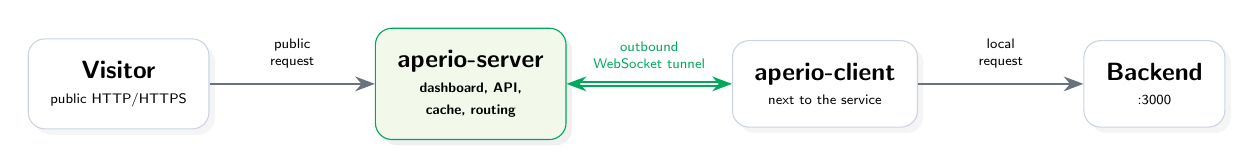
\begin{tikzpicture}[node distance=2.1cm]
  \node[sysnode]                      (visitor) {\textbf{Visitor}\\[-2pt]\tiny public HTTP/HTTPS};
  \node[servernode, right=of visitor] (server)  {\textbf{aperio-server}\\[-2pt]\tiny dashboard, API,\\[-3pt]\tiny cache, routing};
  \node[sysnode, right=of server]     (client)  {\textbf{aperio-client}\\[-2pt]\tiny next to the service};
  \node[sysnode, right=of client]     (backend) {\textbf{Backend}\\[-2pt]\tiny :3000};

  \draw[arrowstd]    (visitor) -- node[edgelabel, above=2pt] {public\\request} (server);
  \draw[arrowtunnel] (client)  -- node[edgelabel, above=2pt, text=AperioGreen] {outbound\\WebSocket tunnel} (server);
  \draw[arrowstd]    (client)  -- node[edgelabel, above=2pt] {local\\request} (backend);
\end{tikzpicture}
\caption{The shape of every deployment: the only arrow that starts on the
private side is the tunnel, and it points outward.}
\end{figure}

Three properties follow from this shape, and most of the rest of the book
is a consequence of one of them:

\begin{enumerate}[leftmargin=1.5em]
  \item \textbf{The client is a client.} It initiates the connection, so
        it can disappear at any moment and reappear from a different
        address. Everything about routing, health and failover exists
        because the serving side is not reliably present.
  \item \textbf{The server is the only shared point.} It is the only
        component that sees all traffic and all clients at once, which is
        why load balancing, caching, statistics and autoscaling decisions
        live there.
  \item \textbf{The tunnel is one connection.} Every request, response,
        WebSocket frame and TCP byte for a service is multiplexed over a
        single WebSocket, which is what makes the protocol
        (Appendix~\ref{app:protocol}) more than a thin pipe.
\end{enumerate}

\section{When not to use it}

Honesty is cheaper than a failed rollout:

\begin{itemize}[leftmargin=1.3em]
  \item If the service can simply be deployed to a public host, deploy it.
        A tunnel adds a hop and a moving part.
  \item If you need raw, high-throughput TCP for a long-lived workload
        (bulk database replication, for instance), the experimental TCP
        support in Chapter~\ref{ch:emergency} is the wrong tool; use a
        VPN or a direct peering.
  \item If the private side genuinely cannot make outbound connections at
        all, nothing here helps.
\end{itemize}

\chapter{Architecture}
\label{ch:architecture}

\section{The life of a request}

Understanding one request end to end explains most of the configuration
surface. A visitor request arrives at the server and passes through the
following stages, in this order. Each stage can end the request.

\begin{enumerate}[leftmargin=1.5em]
  \item \textbf{Per-IP rate limit.} A token bucket keyed on the visitor
        address. Exceeding it answers \code{429} before anything else is
        evaluated.
  \item \textbf{Visitor gate.} If the route is protected by a password,
        by OIDC, or by a client-declared per-service login, an
        unauthenticated visitor is redirected to the login page. Public
        routes and valid share links skip this.
  \item \textbf{Global wait.} If no client at all is connected, the
        request waits, bounded by the gateway timeout, for one to appear.
        This is also where a cold start is triggered when the service
        opted into autoscaling (Chapter~\ref{ch:autoscaling}).
  \item \textbf{Admission.} A server-wide concurrency slot is taken. Over
        the limit answers \code{429}. Note the ordering: the wait above
        happens \emph{before} a slot is held, so visitors waiting for a
        sleeping service cannot starve healthy ones.
  \item \textbf{Route resolution.} The hostname and path select a pool of
        eligible clients; the load-balancing strategy picks one. No pool
        means the stale-cache, fallback and \code{504} chain.
  \item \textbf{Per-client admission.} The chosen client's own
        concurrency limiter is taken, so the server never pushes more
        parallel work at a backend than it announced it can handle.
  \item \textbf{Dispatch.} The request is serialised onto the tunnel. The
        client forwards it to the backend and streams the response back.
  \item \textbf{Response handling.} Header rules, security headers, the
        cache, the request inspector and the access log all see the
        response before the visitor does.
\end{enumerate}

\begin{aperionote}{Why the order matters}
Two stages are deliberately placed where they are. The visitor gate runs
before routing, so an unauthenticated visitor never influences client
selection. Admission runs after the connection wait, so a slow cold start
cannot consume the server's global concurrency budget.
\end{aperionote}

\section{The concurrency model}

Aperio runs on Tokio with one task per tunnel connection, plus one task
per in-flight request. There are three separate concurrency limits, and
confusing them is a common source of unexpected \code{429}s:

\begin{description}[leftmargin=1.6em,style=nextline]
  \item[Server-wide] \code{APERIO\_MAX\_CONCURRENT\_REQUESTS} caps
        in-flight proxied requests across every service. It protects the
        server process itself.
  \item[Per client] The client announces \code{max\_concurrent}; the
        server holds a semaphore of that size and queues beyond it rather
        than flooding the backend. This is also the signal autoscaling
        reads.
  \item[Per visitor] The IP token bucket, which is about abuse rather
        than capacity.
\end{description}

\section{Where state lives}

\begin{longtable}{@{}>{\raggedright\arraybackslash}p{0.30\linewidth}p{0.62\linewidth}@{}}
\toprule
\textbf{State} & \textbf{Where it lives} \\
\midrule
\endhead
Dynamic tokens, users, organisations, webhooks, admin keys, autoscaling
records & \code{aperio.db} (SQLite) in the data directory; survives
restarts \\
Statistics, uptime history, webhook deliveries & the same database,
flushed periodically and on shutdown \\
Audit log & \code{audit.jsonl} plus rotated generations, hash-chained \\
Access log & \code{APERIO\_ACCESS\_LOG} path, one JSON object per line \\
Connected clients, their binds and health & memory only; rebuilt on
every connect \\
Maintenance flags, dashboard bind overrides & memory only; cleared by a
restart \\
Response cache, captured requests, live traffic buffer & memory only,
bounded \\
Dashboard settings overrides & \code{settings.json} in the data
directory; wins over file and environment \\
\bottomrule
\end{longtable}

The split is deliberate. Anything an operator typed is persisted;
anything derived from a live connection is not, because a restart should
never resurrect a stale view of who is serving what.

\section{Trust boundaries}

Four actors, decreasing in trust from right to left:

\begin{figure}[htbp]
\centering
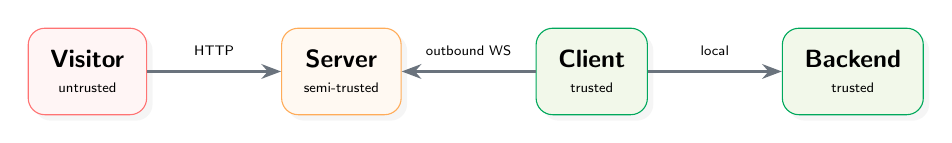
\begin{tikzpicture}[node distance=1.7cm]
  \node[sysnode, draw=red!55, fill=red!4]              (visitor) {\textbf{Visitor}\\[-2pt]\tiny untrusted};
  \node[sysnode, draw=orange!65, fill=orange!5, right=of visitor] (server) {\textbf{Server}\\[-2pt]\tiny semi-trusted};
  \node[sysnode, draw=AperioGreen, fill=AperioGreenLight, right=of server] (client) {\textbf{Client}\\[-2pt]\tiny trusted};
  \node[sysnode, draw=AperioGreen, fill=AperioGreenLight, right=of client] (backend) {\textbf{Backend}\\[-2pt]\tiny trusted};

  \draw[arrowstd] (visitor) -- node[edgelabel, above=2pt] {HTTP} (server);
  \draw[arrowstd] (client)  -- node[edgelabel, above=2pt] {outbound WS} (server);
  \draw[arrowstd] (client)  -- node[edgelabel, above=2pt] {local} (backend);
\end{tikzpicture}
\caption{Four actors, decreasing in trust from right to left. The server is
semi-trusted on purpose.}
\end{figure}

The server is \emph{semi}-trusted on purpose: it terminates visitor TLS
and can see plaintext traffic, so a client that must not trust its server
has one escape hatch, the end-to-end encrypted emergency tunnels of
Chapter~\ref{ch:emergency}. Everything else in the security model assumes
the server is honest but that clients and visitors are not.

\chapter{Getting started}
\label{ch:getting-started}

\section{Run a server}

\begin{codecard}[aperiosh]{On the public box}
docker run -d --name aperio-server \
  -p 8080:8080 \
  -e APERIO_SERVER_TOKEN="change-me-to-a-long-random-string" \
  -v ./data:/app/data \
  ghcr.io/co3moz/aperio-server:latest
\end{codecard}

The token is the master credential: it authenticates tunnel clients and
doubles as the dashboard password. The volume holds the database, so
skipping it means losing every token and statistic on the next restart.

\section{Connect a client}

\begin{codecard}[aperiosh]{On the machine next to the service you are exposing}
aperio-client 3000 \
  --server-url https://tunnel.example.com \
  --server-token apr_xxxxxxxx
\end{codecard}

The positional argument is deliberately forgiving: a bare port becomes
\code{http://localhost:3000}, a bare hostname becomes \code{http://host},
and a full URL passes through untouched.

\section{Verify}

Before debugging anything else, run the built-in diagnostic:

\begin{codecard}[aperiosh]{On the machine next to the service you are exposing}
aperio-client check
\end{codecard}

It resolves the configuration and reports \emph{which layer} supplied each
value, probes the server's health endpoint, compares client and server
versions and protocol numbers, performs a real token handshake, and dials
every local target. Exit code \code{0} means every hop is green. Most
"it does not work" reports are answered by its output alone.

\section{A first real configuration}

Command-line flags are fine for a demo; anything long-lived belongs in a
file:

\begin{codecard}[aperioyaml]{./aperio.yaml (client)}
server:
  url: https://tunnel.example.com
  token: apr_xxxxxxxxxxxxxxxx

services:
  - target: http://localhost:3000
    hostname: app.example.com
    health:
      endpoint: /health    # hold the service out of routing until it answers

# Optional, but worth setting early. Top-level keys are the defaults every
# entry inherits:
max_concurrent: 8          # what one instance of the backend can take
\end{codecard}

A file describes its backends under \code{services:}, even when there is
one of them. Naming a single backend at the top level instead
(\code{target:}, \code{serve:}, \code{hostname:}, \code{path:},
\code{tcp\_target:}, \code{target\_health:}) still works and is
deprecated: it is removed in 0.9.0, and until then a client that finds it
says so at startup. Single-service mode itself is unaffected where it
belongs, on the command line and in the environment.

The file is watched: editing it re-resolves the whole configuration and
respawns the services, so every setting takes effect without a restart.

% =====================================================================
\part{Configuring}
% =====================================================================

\chapter{The configuration model}
\label{ch:config-model}

\section{Three surfaces, one name}

Naming is mechanical across every surface, which is what makes the
reference tables usable. A setting called \code{server.token} in the
client's yaml is \code{APERIO\_SERVER\_TOKEN} in the environment and
\code{--server-token} on the command line. There are no scoping aliases
and no alternate spellings; where a shorthand exists (\code{--server},
\code{--token}, \code{--host}) it is a visible alias of the canonical
flag, not a second setting.

Settings that share a prefix are written as a \emph{block} in yaml, since
a flat list of run-on names reads badly when they are one subject:

\begin{codecard}[aperioyaml]{aperio-server.yaml}
cache:
  enabled: true
  max_bytes: 268435456
\end{codecard}

The environment has no nesting, so the mapping stays mechanical in both
directions: \code{<group>.<child>} is \code{APERIO\_<GROUP>\_<CHILD>}, and
\code{cache.max\_bytes} is still \code{APERIO\_CACHE\_MAX\_BYTES}. Where
the group's own key is also a setting, the child carrying it is
\code{enabled} (or \code{mode} for \code{failover}), and the bare scalar
(\code{cache: true}) is still accepted. The client has \code{health:} (at
the top level and per \code{services:} entry) and the long-standing
\code{server:}; the server has \code{alert}, \code{audit}, \code{cache},
\code{dashboard}, \code{edge}, \code{failover}, \code{gateway},
\code{ip\_limit}, \code{login\_lockout}, \code{metrics}, \code{oidc},
\code{otel}, \code{outbound}, \code{retention}, \code{scaling},
\code{server} and \code{stream}.

Every flat key still works exactly as it did, so no existing file needs
changing; a file may mix both spellings, with the block winning per field,
and the client names the block to move each flat key to.

\section{Precedence}

The two sides layer differently, and both are worth memorising.

\subsection*{Client}

\begin{enumerate}[leftmargin=1.5em]
  \item CLI arguments (highest)
  \item \code{./aperio.yaml}, or the file named by \code{--config}
  \item environment variables
  \item \code{\textasciitilde/.aperio.yaml}, user-level defaults (lowest)
\end{enumerate}

The home file exists so a developer can set the server URL and token once
and keep per-project files down to a target and a hostname.

\subsection*{Server}

\begin{enumerate}[leftmargin=1.5em]
  \item Dashboard overrides in \code{settings.json} (highest, runtime)
  \item \code{aperio-server.yaml}
  \item environment variables (lowest)
\end{enumerate}

The mechanism is worth knowing because it explains the order: at startup
the server reads \code{aperio-server.yaml} and \emph{materialises every
scalar key into its environment variable}, overwriting whatever was
there. So the file always wins, and \code{--print-config} can attribute
each value to its source afterwards.

\begin{aperionote}{Consequence}
Setting a value in both places is not an error and produces no warning:
the file silently wins. When a change to an environment variable appears
to do nothing, look for the key in \code{aperio-server.yaml} first.
\end{aperionote}

\section{Inspecting what is actually set}

Two subcommands answer the two questions operators actually ask.

\code{--check-config} validates the layered configuration without binding
a port or touching the data directory. It parses every numeric and
enumerated value, checks the structured sections, and exits non-zero when
anything is wrong:

\begin{codecard}[aperiosh]{On the aperio-server host}
aperio-server --check-config
\end{codecard}

\code{--print-config} answers "what is in effect, and where did it come
from?". Every \code{APERIO\_*} variable in force is listed and attributed
to either the file or the real environment, secret-looking values are
masked, and the persisted dashboard overrides are shown separately:

\begin{codecard}[aperiosh]{On the aperio-server host}
aperio-server --print-config
\end{codecard}

A third, \code{--print-schema}, emits the machine-readable catalogue of
every setting with its default, which is what the reference appendices of
this book are checked against.

\section{Declaring the version a file targets}
\label{sec:config-version}

Both files take a \code{version:} key naming the Aperio release they were
written against:

\begin{lstlisting}[language=aperioyaml]
version: 0.5.0
\end{lstlisting}

On startup the binary compares it against its own build and looks up every
recorded change to the configuration \emph{format} that landed in between.
The behaviour is deliberately quiet. Nothing in that range means the upgrade
cannot affect this file, and nothing is printed, so silence itself is the
signal. Something in the range prints each change, the keys it touched and
what to do, then asks for \code{version:} to be bumped once reviewed. A
change with security consequences, a default that opens something previously
closed or an enforcement that quietly stopped applying, makes the binary
refuse to start: continuing silently is worse than an outage you can see. A
file declaring a version newer than the binary is called out as well, since a
rollback nobody rolled the config back for may use settings this build has
never heard of.

Leaving the key out keeps the old behaviour exactly, with one line noting the
check is off. The recorded history starts at the release that introduced the
mechanism; entries for older versions could only be guesses, so none are
claimed.

\section{Hot reload}

\code{aperio-server.yaml} is watched. Edits apply live for the
\emph{live-editable} surface, the same set the dashboard can change:
cache, failover, rate limits, lockout, body and concurrency limits, the
stream flow-control watermarks, audit rotation,
\code{require\_hostname\_bind}, tunnel compression, UI language, preview
noindex, visitor auth, plus the structured \code{headers:},
\code{routes:} and \code{error\_pages:} sections. Grouped and flat
spellings are folded identically on reload, so a file written with blocks
reloads exactly like one written flat.

Structural keys are deliberately \emph{not} hot-reloaded and need a
restart: host and port, the data directory, proxy-trust flags, OIDC, the
random-subdomain pattern, the custom error-page file paths, the outbound
callback policy, and \code{expose:} ports. Reloads are audit-logged as
\code{config\_reloaded}.

The watcher is on by default and \code{APERIO\_CONFIG\_HOT\_RELOAD=0}
turns it off, for a deployment that would rather restart deliberately than
have a half-saved file apply itself. \code{APERIO\_SERVER\_CONFIG} points
at the file when it does not sit next to the binary; the name deliberately
differs from the client's \code{aperio.yaml} so the two are never confused.

\section{Editor support}

Building the client emits JSON Schemas for both config files into
\code{schemas/}, so an editor with the YAML extension gives completion and
inline validation for every key in this book:

\begin{codecard}[aperiojson]{.vscode/settings.json}
{
  "yaml.schemas": {
    "./schemas/aperio-client.schema.json": ["aperio.yaml", "**/aperio.yaml"],
    "./schemas/aperio-server.schema.json": ["aperio-server.yaml"]
  }
}
\end{codecard}

\chapter{Configuring the client}
\label{ch:client-config}

\section{What to expose}

A client exposes exactly one of three things per service:

\begin{description}[leftmargin=1.6em,style=nextline]
  \item[A backend URL] \code{target: http://localhost:3000}. Also
        \code{h2c://} or \code{h2://} for HTTP/2 and gRPC backends, and
        \code{unix:///var/run/app.sock} for a Unix domain socket.
  \item[A directory] \code{serve: ./dist} starts a built-in static file
        server. Directories serve their \code{index.html};
        \code{APERIO\_SERVE\_SPA=1} makes navigations fall back to the
        root index, which is what a client-side router needs. Files are
        streamed rather than read into memory, and \code{Range} requests
        are answered, so a large download or a video behaves properly.
  \item[A raw TCP port] \code{tcp\_target:} and the \code{tunnels:} list,
        covered in Chapter~\ref{ch:emergency}.
\end{description}

\section{Binds: hostname and path}

A bind is the client's claim on a slice of the server's traffic. A
hostname bind matches the \code{Host} header; a path bind matches a URL
prefix. Both are validated against the token's permissions, so a client
cannot claim what its credential does not allow.

\begin{codecard}[aperioyaml]{./aperio.yaml (client)}
services:
  - target: http://localhost:3000
    hostname: app.example.com   # or a list: [app.example.com, www.example.com]
    path: /api                  # optional prefix bind
    trim_bind: true             # strip /api before forwarding (default with a path bind)
\end{codecard}

A bind belongs to the service it binds, which is why it is written on the
entry rather than beside it.

\section{Several services from one process}

Add an entry per backend and the client opens one tunnel connection per
entry, each with its own binds, health probe and limits:

\begin{codecard}[aperioyaml]{./aperio.yaml (client)}
server:
  url: https://tunnel.example.com
  token: apr_xxxxxxxxxxxxxxxx
services:
  - name: web
    target: http://localhost:3000
    hostname: app.example.com
    target_health: /health
  - name: api
    target: http://localhost:4000
    hostname: api.example.com
    max_concurrent: 32
  - name: docs
    serve: ./site
    hostname: docs.example.com
\end{codecard}

Per-entry keys override the top-level value entirely rather than merging,
which keeps the mental model simple: a service either declares a setting
or inherits it.

\section{Editing traffic}

Two mechanisms, applied on the client side of the tunnel:

\begin{codecard}[aperioyaml]{./aperio.yaml (client)}
headers:
  request:                       # what the local backend receives
    add:
      X-Forwarded-Env: staging
    remove: [X-Internal-Debug]
  response:                      # what the visitor receives
    add:
      X-Served-By: aperio
    remove: [Server, X-Powered-By]

security_headers: true           # HSTS, X-Frame-Options, nosniff, Referrer-Policy
\end{codecard}

\code{security\_headers} also takes a mapping when the standard preset is
too much, and \code{false} on a service opts it out of a top-level
preset. Hop-by-hop and tunnel-critical headers stay managed by Aperio no
matter what the rules say.

\section{Capacity and resilience knobs}

The four that matter most in production:

\begin{description}[leftmargin=1.6em,style=nextline]
  \item[\code{max\_concurrent}] What one instance of the backend can
        handle at once. The server queues beyond it instead of flooding,
        and autoscaling measures saturation against it. Setting it is the
        difference between a backend that degrades gracefully and one
        that falls over.
  \item[\code{target\_health}] A path the client probes; while it fails,
        the service is held out of routing without dropping the tunnel.
  \item[\code{connections}] Parallel tunnel connections per service. More
        connections mean a dropped one is covered by a sibling with no
        visitor-facing gap.
  \item[\code{priority}] Load-balancing tier. \code{0} is primary, higher
        is standby, which only matters under the primary-standby strategy.
\end{description}

\chapter{Configuring the server}
\label{ch:server-config}

\section{The minimum}

\begin{codecard}[aperioyaml]{aperio-server.yaml}
server_token: change-me-to-a-long-random-string   # env: APERIO_SERVER_TOKEN
port: 8080                                        # env: PORT
data_dir: /app/data                               # env: APERIO_DATA_DIR
trust_proxy: true                                 # env: APERIO_TRUST_PROXY
\end{codecard}

\code{trust\_proxy} deserves a sentence of its own: it tells the server to
believe forwarded-for headers when resolving the visitor address. Enable
it when, and only when, something you control terminates TLS in front,
and pair it with \code{trusted\_proxies} so the real address is resolved
by walking the chain rather than trusting the first hop blindly.

\section{Structured sections}

Beyond scalar settings the file carries five structured sections. They are
not expressible as environment variables, which is the main reason to use
the file at all.

\subsection{Static routes}

A hostname or path answered by the server itself, with no client involved.
Useful for vanity redirects, a placeholder for a service that is not
deployed yet, or a fixed \code{robots.txt}:

\begin{codecard}[aperioyaml]{aperio-server.yaml}
routes:
  - hostname: old.example.com
    redirect: https://new.example.com
    permanent: true
    preserve_path: true
  - hostname: soon.example.com
    respond:
      status: 503
      content_type: text/html
      body: "<h1>Launching next week</h1>"
\end{codecard}

Routes match before client routing; maintenance mode still wins over them.
They serve operator-authored content, so the visitor gate does not apply.

An entry with neither \code{redirect} nor \code{respond} is a \emph{policy}
rule instead of an answer: it does not end the request, it configures the
proxied traffic that matches it. \code{timeout} overrides the response
timeout for that route, \code{headers} adds request and response edits on top
of the server-wide \code{headers:} section, and \code{rate\_limit} carries the
same fields as a \code{rate\_limits:} rule without repeating the hostname and
path:

\begin{codecard}[aperioyaml]{aperio-server.yaml}
routes:
  - path: /uploads
    timeout: 600
    rate_limit:
      rps: 2
      methods: [POST]
  - hostname: cdn.example.com
    path: /static
    headers:
      response:
        add:
          cache-control: "public, max-age=3600"
\end{codecard}

The two kinds are matched independently, each first-match in file order, and
cannot be combined on one entry: a static answer never reaches a backend, so
backend policy on it would be silently meaningless, and the server says so at
startup instead.

\subsection{Scheduled maintenance windows}

Maintenance mode is a switch an operator flips, with an optional TTL, which
covers the unplanned outage. A window that comes round every week is standing
configuration instead, so it is written in the config file: there it survives
a restart, which the in-memory runtime flags do not, reloads without one, and
is reviewed in a diff.

\begin{codecard}[aperioyaml]{aperio-server.yaml}
maintenance_windows:
  - hostname: "*.example.com"
    from: "02:00"
    to: "04:00"
    days: [sat, sun]
    tz: Europe/Istanbul
    reason: weekly patching
\end{codecard}

While a window runs, matching hostnames answer exactly as a flag would, with
\code{Retry-After} pointing at the end of the window. A \code{to} earlier
than \code{from} wraps past midnight, and \code{days} then names the day the
window \emph{starts}. The zone is an IANA name rather than a fixed offset, so
02:00 stays 02:00 across a daylight-saving change.

\subsection{Fallbacks}

Where a static route answers instead of a client, a fallback answers
instead of a \code{504} when no client is currently serving a hostname:

\begin{codecard}[aperioyaml]{aperio-server.yaml}
fallbacks:
  - hostname: app.example.com
    url: https://status.example.com
  - hostname: "*"
    url: https://www.example.com
    preserve_path: true
\end{codecard}

\subsection{Route rate limits}

Per-route caps, aggregated across all visitors, for endpoints that are
expensive or attractive to attackers:

\begin{codecard}[aperioyaml]{aperio-server.yaml}
rate_limits:
  - hostname: app.example.com
    path: /login
    rps: 5
    burst: 10
  - path: /api/items
    rps: 2
    methods: [POST, PUT, DELETE]
\end{codecard}

An optional \code{methods:} list scopes a rule to those verbs, so a write path
is throttled while reads of the same route are not. Rules differing only by
method own separate buckets.

\subsection{Request firewall}

A small rule list evaluated before dispatch. Each rule matches a path
regex, a set of methods, or a header regex:

\begin{codecard}[aperioyaml]{aperio-server.yaml}
waf:
  - path: "^/\\.git"                 # block probes for an exposed repository
  - path: "^/admin"
    methods: [POST, PUT, DELETE]
  - header:
      name: user-agent
      regex: "(?i)sqlmap|nikto"
\end{codecard}

\subsection{Per-hostname error pages}

\begin{codecard}[aperioyaml]{aperio-server.yaml}
error_pages:
  - hostname: app.example.com
    504_page: ./pages/app-504.html
    503_page: ./pages/app-503.html
\end{codecard}

\section{Choosing limits}

Defaults are chosen to be safe rather than fast. Three worth revisiting
before a launch:

\begin{itemize}[leftmargin=1.3em]
  \item \code{APERIO\_MAX\_CONCURRENT\_REQUESTS}, the global in-flight
        ceiling. Too low and bursts get \code{429}; too high and a slow
        backend can exhaust memory with queued bodies.
  \item \code{APERIO\_MAX\_BODY\_SIZE}, the largest request body accepted.
        Clients can lower it per service; they cannot raise it.
  \item \code{APERIO\_GATEWAY\_TIMEOUT}, how long a request waits for a
        client to appear. Raising it hides client instability; lowering it
        surfaces it as \code{504}s.
\end{itemize}

% =====================================================================
\part{Traffic}
% =====================================================================

\chapter{Routing and load balancing}
\label{ch:routing}

\section{Eligibility comes first}

Before any strategy runs, the pool is filtered to clients that could
actually take a request. A client is eligible when its heartbeat is
recent, its backend health probe passes, it is not draining, it has not
been disabled from the dashboard, and it has not been ejected as an
outlier. Everything else in this chapter operates on what survives that
filter.

\section{Binds}

A request is matched to a pool by hostname first, then by path prefix.
The rules are deliberately boring:

\begin{itemize}[leftmargin=1.3em]
  \item An exact hostname match wins over a client with no hostname bind.
  \item A path bind matches a prefix at a segment boundary, so
        \code{/api} matches \code{/api/v1} but not \code{/apiary}.
  \item A client with no bind at all is a catch-all, which is why
        \code{APERIO\_REQUIRE\_HOSTNAME\_BIND=1} exists: in a
        multi-tenant deployment a catch-all is almost always a mistake.
\end{itemize}

\section{Strategies}

\begin{description}[leftmargin=1.6em,style=nextline]
  \item[\code{round-robin}] The default. Requests rotate across the
        eligible pool.
  \item[\code{primary-standby}] Only tier \code{0} clients serve while any
        of them is eligible; higher tiers take over when they are all
        gone. This is the shape you want for a warm spare.
  \item[\code{sticky}] A returning visitor carries an affinity cookie
        naming the client that served them last, and goes back to it while
        it stays eligible. Session affinity for applications that keep
        per-instance state.
\end{description}

\section{Random subdomains}

With a wildcard pattern configured, every connecting client is also
assigned a generated hostname:

\begin{codecard}[aperioyaml]{aperio-server.yaml}
random_subdomain: "*.example.com"    # env: APERIO_RANDOM_SUBDOMAIN
preview_noindex: true                # env: APERIO_PREVIEW_NOINDEX
\end{codecard}

The label is derived deterministically from the client's instance group
and declared binds, so every parallel connection of one process converges
on the \emph{same} generated name instead of each minting its own. That
detail matters for \code{connections: N}: without it a service with four
tunnel connections would answer on four different preview URLs.

\code{preview\_noindex} answers a real operational problem: preview URLs
are public and crawlers do find them. With it set, services reached
through a generated subdomain answer with \code{X-Robots-Tag: noindex}
and a disallow-all \code{robots.txt}. Explicitly named hostnames are
treated as deliberate and are never marked.

\section{Dashboard overrule}

An operator can point a hostname or path at a specific connected client
from the dashboard, overriding what the client declared. It is in-memory
and disappears when the client reconnects, which makes it the right tool
for a one-off investigation and the wrong tool for configuration.

\section{Passive outlier ejection}

A client that crosses a failure threshold (5xx responses, timeouts,
connection loss) is silently pulled from rotation while its tunnel stays
up, then allowed back. This is the one routing behaviour that is
invisible from the client's side, which is why the topology view and the
client detail both surface an \code{ejected} flag.

\chapter{In-flight failover}
\label{ch:failover}

\section{The window}

Failover only ever applies while \textbf{no response bytes have reached
the visitor}. Once the first byte is out, the only honest thing to do is
fail, because a retry would produce a spliced response. Everything below
happens inside that window.

\section{Modes}

\begin{longtable}{@{}>{\raggedright\arraybackslash}p{0.20\linewidth}p{0.72\linewidth}@{}}
\toprule
\textbf{Mode} & \textbf{Behaviour} \\
\midrule
\endhead
\code{fail} & Answer \code{502} immediately. The default. \\
\code{retry} & Re-dispatch to another currently eligible client; fail when
there is none. \\
\code{wait} & Wait for the \emph{same} client instance to reconnect and
re-dispatch to it. Right for a single client that restarts. \\
\code{retry-wait} & Re-dispatch if another candidate exists, otherwise
wait. \\
\bottomrule
\end{longtable}

\section{Guards}

Two bounds keep failover from becoming an amplifier:
\code{APERIO\_FAILOVER\_MAX\_JUMPS} caps how many times one request may be
re-dispatched, and \code{APERIO\_FAILOVER\_WINDOW} caps how long the whole
sequence may take from the first failure.

By default only idempotent methods are re-dispatched. Setting
\code{APERIO\_FAILOVER\_ALL\_METHODS=1} includes \code{POST}, which is
safe only if your handlers are idempotent, and is a decision to make
deliberately rather than by default.

\begin{aperionote}{Not the same as a cold start}
Failover governs a request that was already dispatched. A request that
never found a client at all is a different path entirely, and is where
autoscaling hooks in (Chapter~\ref{ch:autoscaling}). Because such a
request was never sent anywhere, holding it is safe for every method, so
the idempotency rules above deliberately do not apply to it.
\end{aperionote}

\chapter{Response caching}
\label{ch:caching}

\section{The two-key opt-in}

The cache never turns on by accident. It requires \emph{both}:

\begin{codecard}[aperioyaml]{aperio-server.yaml}
cache: true                    # env: APERIO_CACHE
\end{codecard}

\begin{codecard}[aperioyaml]{./aperio.yaml (client)}
cache: true                    # per service, or top-level
\end{codecard}

The operator enables the machinery; the service owner opts their service
in. A service that opts in against a disabled cache is not silently
ignored: the server logs a one-time warning and the dashboard marks the
connection \code{cache off}.

\section{What gets cached}

Only \code{GET}, only successful responses, and only when the backend's
\code{Cache-Control} says so. Aperio does not invent freshness. Responses
carrying \code{Set-Cookie}, \code{Authorization}-varying content, or
\code{no-store} are never cached.

\section{What the cache does beyond storing}

Four behaviours matter operationally:

\begin{description}[leftmargin=1.6em,style=nextline]
  \item[Edge 304] A conditional request with a matching \code{ETag} is
        answered from the cache without touching the tunnel.
  \item[Single flight] Concurrent misses for the same key coalesce into
        one backend fetch, so a cold cache under load does not stampede.
  \item[Stale while revalidate] A stale entry can be served immediately
        while a refresh happens in the background.
  \item[Serve stale] With \code{resilience: true} on the service, cached
        answers keep being served (marked, even expired) while no healthy
        client is connected, instead of a \code{504}.
\end{description}

\section{Invalidation}

\begin{codecard}[aperiosh]{From anywhere, against the server's admin API}
aperio-client api cache purge --hostname app.example.com --path-prefix /assets/
aperio-client api cache purge --surrogate-key build-7
\end{codecard}

Surrogate keys come from a backend \code{Surrogate-Key} response header
and give CDN-style tag invalidation: deploy, purge the tag, done.

\chapter{Protocols and streaming}
\label{ch:protocol-chapter}

\section{What travels over one connection}

A single WebSocket carries every kind of traffic for a service,
multiplexed by request id. The full message catalogue is
Appendix~\ref{app:protocol}; the shapes that matter here are:

\begin{itemize}[leftmargin=1.3em]
  \item Buffered requests and responses, for ordinary small payloads.
  \item Chunked streams (\code{RequestStart}/\code{Chunk}/\code{End} and
        the response equivalents), so a large upload or download never
        has to be held in memory on either side.
  \item WebSocket pass-through, where the visitor's upgrade is relayed and
        frames flow in both directions.
  \item Raw TCP and UDP relays for emergency tunnels; since v7 their
        payloads travel as binary frames rather than base64 in JSON, as
        does a binary WebSocket frame.
  \item Per-stream flow control (\code{StreamPause}/\code{StreamResume}),
        which lets the server throttle one producer without touching
        anything else on the connection.
  \item Messages between clients (\code{Subscribe}/\code{Publish} and
        their acknowledgements), Chapter~\ref{ch:messaging}.
\end{itemize}

Since protocol v5 a buffered response body travels as bytes in the same
binary frame as its JSON envelope rather than base64 inside it, and
since v6 a buffered request body does too; the change is negotiated, so
an older peer on either side keeps receiving base64 in JSON.

\section{HTTP/2 and gRPC}

A target of \code{h2c://} or \code{h2://} makes the client dial the
backend over HTTP/2 with prior knowledge. \code{te: trailers} is
forwarded and response trailers such as \code{grpc-status} are relayed
back, which is what makes gRPC work end to end. The visitor leg must also
be HTTP/2 for trailers to survive, so whatever fronts Aperio has to
forward gRPC as HTTP/2 rather than downgrading it.

\section{Compression}

When the server offers it and the client acknowledges, tunnel frames are
zlib-compressed. This is compression \emph{of the tunnel}, independent of
any \code{Content-Encoding} the backend sets, and it is negotiated at
connect time rather than configured on both sides.

\section{Binary frames}

Protocol v2 moves chunk payloads to binary WebSocket frames with a compact
\code{[tag][id\_len][id][payload]} header, instead of base64 inside JSON.
The parser for those frames is the primary untrusted-input surface in the
system, which is why it is fuzzed continuously
(Chapter~\ref{ch:troubleshooting} covers running the fuzzers).

\section{Flow control}
\label{sec:flow-control}

The current protocol version is 7. Version 3 added flow control for
everything that streams; version 5 moved a buffered response body out of
JSON and into the frame that carries its envelope, version 6 did the same
for a buffered request body, in the direction an upload travels, and
version 7 did it for the relay payloads, the last leg that was still
base64.

The awkward case is a visitor who reads more slowly than the backend
produces. One connection's read loop is shared by every request and stream
on it, so the server must never block waiting on a single consumer; but it
cannot buffer without bound either, and cutting the stream would kill a
download that is perfectly healthy, merely slow. So the server pushes back
on the producer instead. It counts the bytes queued for each stream, and
past \code{APERIO\_STREAM\_PAUSE\_BYTES} (2\,MB by default) it sends
\code{StreamPause} for that stream id. The client stops reading that one
stream's source, the backend response body, the backend WebSocket or the
TCP socket, so ordinary TCP backpressure reaches the backend, which is
where it belongs. When the backlog falls below
\code{APERIO\_STREAM\_RESUME\_BYTES} (512\,KB) a \code{StreamResume}
follows. The two marks sit far apart on purpose, so the pair cannot flap
chunk by chunk.

Everything else on the tunnel keeps flowing while one stream is paused:
other visitors' responses, other streams, the heartbeat. UDP relays are
deliberately excluded and keep their drop-when-congested contract.

Two bounds keep the mechanism honest. A producer that cannot be paused,
an older client, or one that ignores the pause, is cut off at
\code{APERIO\_STREAM\_BACKLOG\_LIMIT} (16\,MB) of buffered bytes; and a
consumer that accepts nothing at all for the whole response timeout still
ends its own stream, exactly as before. On the client side a stream that
has been paused for more than thirty seconds resumes by itself, so a
resume lost along with a torn-down stream cannot wedge a producer.

The watermarks are server settings. An inconsistent trio is repaired
rather than obeyed: the resume mark is kept below the pause mark and the
hard cap above it, so the feature cannot be configured into dropping every
stream. Each stream snapshots the values when it starts, so a change
applies to streams opened after it.

% =====================================================================
\part{Security}
% =====================================================================

\chapter{Tokens and authentication}
\label{ch:tokens}

\section{The master token}

\code{APERIO\_SERVER\_TOKEN} is root. It authenticates any tunnel client
without restriction, logs into the dashboard as the built-in \code{aperio}
admin, authorises the programmatic tunnel API, and derives the signing key
for share links. Treat it as a root password: never put it in a client
that only needs to serve one hostname, and never let it travel in
plaintext.

\section{Dynamic tokens}

The credential you should actually hand out. Each carries:

\begin{description}[leftmargin=1.6em,style=nextline]
  \item[Hostname and path permissions] What the holder may bind.
        \code{*} or an empty list means unrestricted \emph{within the
        organisation's fence}.
  \item[Source IP allowlist] Which addresses may connect with it.
  \item[Lifetime] An optional TTL. Expired tokens are refused at connect.
  \item[Rate limit and daily quota] Applied to the traffic served through
        the token, not to the token's own use.
  \item[\code{allow\_public}] Whether clients using it may publish a
        service as public, skipping the server's visitor gate.
  \item[\code{canary}] A decoy: any successful authentication raises an
        alert. A token that should never be used is a cheap tripwire.
\end{description}

\begin{codecard}[aperiosh]{From anywhere, with an admin key}
aperio-client api token create --name ci \
  --hostname preview.example.com \
  --allowed-ip 10.0.0.0/8 \
  --expire 30d --max-rps 50
\end{codecard}

\section{Rotation and refresh}

Two different operations that are often confused:

\textbf{Rotation} replaces a token's secret while keeping its identity,
permissions and limits. The old secret keeps working for a grace window so
running clients can migrate without a hard cutover:

\begin{codecard}[aperiosh]{From anywhere, with an admin key}
aperio-client api token rotate <id> --grace 1h
\end{codecard}

\textbf{Refresh} slides a TTL token's expiry forward by its original
lifetime, and authenticates with the token secret itself rather than an
admin credential. That is what lets a long-running CI job keep a
short-lived token alive without holding anything more powerful:

\begin{codecard}[aperiosh]{From anywhere holding the token, e.g. the CI job that uses it}
aperio-client api token refresh --secret apr_...
\end{codecard}

\section{Token pinning}

With \code{APERIO\_TOKEN\_PINNING=1}, the first client device key seen for
a token is pinned, and a later connection presenting a different key, or
none at all, is refused. A leaked token replayed from another machine
cannot serve. Enabling it means every client must carry a device key, so
it is a deployment-wide decision.

\section{Admin keys}

Distinct from tunnel tokens: an admin key is a programmatic credential for
the \emph{dashboard API}, carrying a role (viewer, operator, admin) and an
organisation. It is what \code{aperio-client api ...} authenticates with,
and it can never open a tunnel.

\chapter{Protecting proxied traffic}
\label{ch:visitor-auth}

\section{Three gates, one decision}

A visitor reaching a proxied site meets at most one gate, chosen in this
order of specificity:

\begin{enumerate}[leftmargin=1.5em]
  \item A \textbf{client-declared per-service login}
        (\code{visitor\_auth: user:password}), if the token permits it and
        the server has not set \code{APERIO\_IGNORE\_CLIENT\_AUTH}.
  \item The server's own \textbf{visitor password}
        (\code{APERIO\_SERVER\_AUTH}) or \textbf{OIDC} configuration.
  \item Nothing, if the service declared itself \code{public} and its
        token allows that.
\end{enumerate}

A service is only public when \emph{every} client in its serving pool
agrees; a mixed pool falls back to the gate. The same all-must-agree rule
applies to client-declared credentials, so a request can never be gated
by, or slip past, an override that only some pool members set.

\section{OIDC}

Point Aperio at an identity provider and unauthenticated visitors are
redirected to it; the verified email from the provider's userinfo endpoint
is checked against an allowlist of exact addresses, \code{*@domain}
patterns, or \code{*}. Organisations can bring their own issuer, which is
covered in Chapter~\ref{ch:organizations}.

\section{Share links}

A share link hands out temporary access without creating an account. The
token is JWT-shaped, carries the hostname, an optional path prefix and an
expiry, and is signed with a key derived from the master token:

\begin{codecard}[aperiosh]{From anywhere, with an admin key}
aperio-client api share --hostname app.example.com --path /docs --expire 1d
\end{codecard}

The design is stateless by choice, and the trade-off is worth stating
plainly: links survive restarts because there is no table to lose, but an
individual link \emph{cannot be revoked}. It expires, or you rotate the
master token and invalidate every outstanding link at once. Scope links
to a path and the shortest useful lifetime.

\section{Network fences}

Three blunt but effective controls:

\begin{itemize}[leftmargin=1.3em]
  \item \code{denied\_ips:} refuses a set of source addresses
        everything the server answers, before any other rule runs. It is
        the inverse of the allowlists below, and the one to reach for when
        a single address is abusing the server: an allowlist would lock
        out everyone the operator did not think to name. It hot-reloads,
        so a block takes effect without a restart.
  \item \code{APERIO\_ADMIN\_ALLOWED\_IPS} fences the dashboard and its
        API to a set of source addresses. The login page and the auth
        endpoints stay reachable so password-gated \emph{sites} keep
        working from anywhere.
  \item A client's \code{allowed\_ips} restricts who may reach the
        service it serves. A visitor rejected by every candidate gets the
        \code{denied:} redirect, or a stealth answer identical to an
        unclaimed route, so a blocked address cannot even confirm the
        route exists.
\end{itemize}

\chapter{Organisations and multi-tenancy}
\label{ch:organizations}

\section{The model}

One server, several isolated tenants. There is always exactly one implicit
\textbf{master} organisation, represented internally as "no organisation";
child organisations are stored records. Everything created while an
organisation is selected belongs to it: tokens, users, and through those
tokens, the connected clients and all their traffic.

\section{What is isolated}

Clients, tokens, users, sessions, traffic logs, statistics, uptime
history, webhooks, the webhook inbox, audit events, maintenance flags,
captured requests, and autoscaling records. A named admin signing into a
child organisation sees a self-contained view and nothing else.

\section{What stays global}

Server settings, the response cache (keyed by host and URI, not by
tenant), the expose ports, and organisation management itself. These are
master-only by design.

\section{Quotas}

Each child organisation can carry caps on connected clients, dynamic
tokens, dashboard users, and proxied bytes per calendar month. They are
enforced at the point of creation and, for the byte cap, on each proxied
request against the current month's usage:

\begin{codecard}[aperiosh]{From anywhere, with an admin key}
aperio-client api org quota <id> --max-clients 10 --max-tokens 20 --max-bytes-month 0
\end{codecard}

\section{The hostname allowlist}

Quotas bound how much a tenant can use; the allowlist bounds \emph{what}
it can claim. Without one, a token carrying \code{*} may bind any hostname
on the server, so an organisation admin minting a wildcard token for their
own tenant could claim another tenant's hostname:

\begin{codecard}[aperiosh]{From anywhere, with an admin key}
aperio-client api org create --name Acme --hostname acme.com,*.acme.example.com
\end{codecard}

An entry takes one of three shapes. An exact hostname matches itself. A
subdomain wildcard (\code{*.acme.com}) matches any depth of subdomain but
not \code{acme.com} itself, so an operator who wants both lists both. A
partial leftmost label (\code{*-pi.acme.com}, \code{dev-*.acme.com})
matches one label around the placeholder, which is what a fleet naming
convention looks like: an organisation that owns every
\code{<name>-pi.acme.com} can say exactly that rather than be handed the
whole domain. One placeholder, leftmost label only, the same shape
\code{random\_subdomain} accepts. The fence is enforced at every point a
hostname can be claimed, not once:

\begin{itemize}[leftmargin=1.3em]
  \item token creation and editing refuse an out-of-fence permission;
  \item \textbf{client connect re-checks every declared and token-granted
        bind}, which is the check that actually holds, because a token
        minted before the fence existed cannot bind past it;
  \item ephemeral tunnel provisioning refuses an out-of-fence hostname;
  \item the dashboard bind override refuses one too, the single place a
        bind is set with no token permission behind it.
\end{itemize}

A server-assigned random subdomain is exempt: the tenant cannot influence
which name it gets, so it can never collide with another tenant's
hostname. The master organisation is never fenced.

\chapter{Threat model and hardening}
\label{ch:threat}

\section{What each side is trusted to do}

\begin{longtable}{@{}>{\raggedright\arraybackslash}p{0.18\linewidth}p{0.74\linewidth}@{}}
\toprule
\textbf{Actor} & \textbf{Assumption} \\
\midrule
\endhead
Visitor & Fully untrusted. May forge headers, replay links, probe paths,
and script abuse. \\
Server & Semi-trusted. Terminates TLS and sees plaintext. A client that
cannot accept this uses end-to-end encrypted tunnels. \\
Client & Trusted by its operator, \emph{not} by the server. Its
declarations are validated against its token every time. \\
Backend & Trusted by the client that dials it. \\
\bottomrule
\end{longtable}

The pattern to notice: everything a client says about itself, its binds,
its public flag, its visitor credentials, its scaling declaration, is a
\emph{request} that the server validates against the token, never a fact
the server accepts.

\section{Pre-flight checklist}

\begin{enumerate}[leftmargin=1.5em]
  \item Front the server with TLS. Set \code{trust\_proxy} and
        \code{trusted\_proxies} so visitor addresses are resolved
        correctly rather than trusted blindly.
  \item Replace the master token in every client with a scoped dynamic
        token. Keep the master token for administration only.
  \item Fence the admin surface with \code{APERIO\_ADMIN\_ALLOWED\_IPS}.
  \item Give each organisation a hostname allowlist if you host tenants.
  \item Set retention policies for captures, access log, audit and stats
        to match your data-protection obligations.
  \item Enable the audit log and check
        \code{GET /aperio/api/audit/verify} periodically: it verifies the
        hash chain across all generations and names any broken line.
  \item Decide about token pinning and canary tokens.
  \item Back the database up. \code{aperio-client api export} produces a
        JSON dump of tokens, webhooks, users, organisations and scaling
        records; \code{--include} adds the history the store also holds
        (\code{statistics}, \code{uptime}, \code{inbox},
        \code{admin\_keys}) or narrows the dump to the sections named.
\end{enumerate}

\section{Secrets and redaction}

Credential headers and secret-looking body fields are masked before
anything leaves the server: the request inspector, the cURL copy and the
HAR download all show \code{[REDACTED]}, while the raw capture stays in
memory so replay still re-sends the original bytes. Configuration values
whose key name looks secret are masked in \code{--print-config}. Webhook
signing secrets, scaling secrets and admin keys are write-only: the API
reports whether one is set, never what it is.

% =====================================================================
\part{Operations}
% =====================================================================

\chapter{The dashboard}
\label{ch:dashboard}

The dashboard lives at \code{/aperio} and is a React application embedded
into the server binary; there is nothing extra to deploy. Sign in as
\code{aperio} with the master token, with a separate dashboard password,
as a named user, or through OIDC.

\section{What each screen is for}

\begin{description}[leftmargin=1.6em,style=nextline]
  \item[Overview] Live request rate, totals, connected clients. The
        activity chart answers two questions rather than one: the
        minute-long view is derived in the browser from successive polls,
        so it moves with the traffic and starts empty on a reload, while
        the quarter-hour view is the server's own ring of five-second
        slices and survives one.
  \item[Clients] Every tunnel connection with its binds, version, health,
        concurrency and flags (draining, ejected, cache off). The kill
        switch and bind overrule live here.
  \item[Live Traffic] Requests as they complete, as a table or a console.
        Backed by a server-sent event stream rather than polling.
  \item[Webhook Inbox] Inbound POSTs captured for services that opted in,
        browsable and re-firable.
  \item[Topology] The routing map: clients, routes that exist without a
        client, declared-but-offline binds, and public expose ports.
        It also carries \emph{explain}: name a hostname and a path, and
        the server walks the same decisions the proxy makes, in the same
        order, and marks the one that would answer. It sends nothing, so
        it spends no rate limit and wakes no scaled-to-zero service; when
        nothing serves the route it names the clients that could have and
        why they did not.
  \item[Maintenance] The per-hostname 503 switch. An entry is a hostname,
        a \code{*.example.com} subdomain wildcard (every subdomain, not the
        apex, so an operator who wants both lists both), a partial leftmost
        label (\code{*-pi.example.com}), or \code{*} for the whole server,
        which is master's alone. A flag carries a reason,
        shown to the visitor on the 503 page and to the next operator in
        the list, and optionally a window after which it lifts by itself,
        which also makes \code{Retry-After} truthful. Flags live in memory
        and a restart clears them.
  \item[Autoscaling] Armed records with live pool utilisation
        (Chapter~\ref{ch:autoscaling}).
  \item[Tokens] The management surface for tunnel credentials, mirroring
        the API endpoint behind it.
\end{description}

\section{Two dialogs, not eight pages}

The screens above are places you go and stay. The rest are not, and they
open as dialogs over whatever page you were on rather than replacing it.

\textbf{Settings} holds server settings, organisations, users, webhooks
and the webhook inbox: things you open, change, and leave. \textbf{Tools}
holds the audit log, the API explorer and the config builder: instruments
you reach for when something needs working out. Neither appears in the
URL, so a reload returns to the page underneath with the dialog shut,
which is why a settings form with unsaved edits asks before it is
discarded, on closing, on switching panes, and on the browser's own
reload.

\section{What the settings screen can change}

Everything on it is live: a save applies to the running server with no
restart and no reconnect. The environment and \code{aperio-server.yaml}
provide the defaults; an edit becomes a persisted override in
\code{settings.json} that wins over both and can be reset per field. The
settings are grouped by what they govern: gateway timeouts and body
size; capacity and the client-down threshold; load balancing and the
whole failover policy; the per-IP rate limit; tunnel compression, the
random-subdomain pattern and preview \code{noindex}; the response cache
and its serve-stale window; the stream flow-control watermarks; login
lockout and audit rotation; and the visitor-facing language, password
gate and custom 504/503 pages. Two of them reach connected clients
immediately: enabling compression is offered to them at once, and a new
subdomain pattern re-issues their random hostnames on the spot.

What is \emph{not} there is the point of the design. The master token,
host and port, the data directory, proxy trust, cookie security, OIDC,
metrics, the access log and the outbound callback policy never become
dashboard overrides, because a compromised dashboard session must not be
able to move them. They are settable from the file and need a restart,
and the screen lists them read-only with their current values rather
than hiding them.

\section{Finding a setting}

\code{Ctrl+K} (\code{Cmd+K} on macOS) searches the settings as well as
the pages. A setting matches on its name in either language,
its environment key and its group, and carries its current value, marked
when that value is an override rather than the environment default;
picking one opens the pane, expands the group and scrolls to it. Values
are shown to the master super-admin alone, since only they may read them.

\section{The request inspector}

Any captured request can be opened to see headers, body, the response,
and a per-stage timing breakdown. From there it can be replayed through
the tunnel, copied as cURL, or downloaded as HAR. Secrets are redacted in
all three (see Chapter~\ref{ch:threat}), while replay still sends the
original bytes.

\chapter{The admin API and CLI}
\label{ch:api-cli}

\section{One surface, two front ends}

Everything the dashboard does is an HTTP call under \code{/aperio/api/}.
The whole surface is described by a generated OpenAPI 3.1 document at
\code{GET /aperio/api/openapi.json}, and \code{aperio-client api ...} is
that API on the command line. Appendix~\ref{app:endpoints} lists every
endpoint with the credential it expects.

\section{Authenticating}

The CLI uses a programmatic admin key:

\begin{codecard}[aperioyaml]{./aperio.yaml (client)}
server:
  url: https://tunnel.example.com
  token: apr_...      # tunnel token, for exposing services
  api_key: apk_...    # admin key, for `aperio-client api ...`
\end{codecard}

When no admin key is configured the tunnel token is sent instead. The
server honours it only where the master token is a valid credential, that
is \code{api tunnel create} and \code{delete}, so a CI job that only
provisions preview tunnels needs no admin key at all.

\section{The shape of every command}

One call per invocation. The server's JSON answer is pretty-printed on
stdout and the exit code is \code{0}; an authentication failure, a
non-2xx status or a transport error prints to stderr and exits \code{1}.
Logs go to stderr, so piping into \code{jq} is always safe:

\begin{codecard}[aperiosh]{From anywhere, with an admin key}
TUNNEL="$(aperio-client api tunnel create --name "pr-$PR" --expire 2h)"
export APERIO_SERVER_TOKEN="$(printf '%s' "$TUNNEL" | jq -r .token)"
echo "Preview: $(printf '%s' "$TUNNEL" | jq -r .url)"
\end{codecard}

Lifetimes take human durations (\code{45s}, \code{30m}, \code{2h},
\code{1d}, \code{2w}, \code{never}) and are validated before any request
is sent. The host and path scope reuses the client's own
\code{--hostname} and \code{--path} flags rather than inventing new ones.
Passwords and JSON documents accept \code{-} to read from stdin, so a
secret never lands in shell history.

\section{Command groups}

\code{share}, \code{token}, \code{tunnel}, \code{maintenance},
\code{client}, \code{cache}, \code{webhook}, \code{inbox}, \code{user},
\code{org}, \code{admin-key}, \code{scaling}, \code{request},
\code{settings}, \code{audit}, plus the read-only reports (\code{stats},
\code{history}, \code{uptime}, \code{logs}, \code{topology},
\code{bandwidth}, \code{slow-endpoints}, \code{route-trends},
\code{stage-stats}, \code{self-health}, \code{health},
\code{traffic-csv}) and the data commands (\code{purge}, \code{export},
\code{import}, \code{openapi}).

\chapter{Observability}
\label{ch:observability}

\section{Metrics}

\begin{codecard}[aperioyaml]{aperio-server.yaml}
metrics: true                  # env: APERIO_METRICS
metrics_token: a-long-secret   # env: APERIO_METRICS_TOKEN
\end{codecard}

The endpoint is never public: without an explicit token one is generated
and persisted on first start. Per-tenant counters carry \code{token} and
\code{hostname} labels, which is what makes quota and billing dashboards
possible.

\section{Tracing}

\begin{codecard}[aperioyaml]{aperio-server.yaml}
otel:
  enabled: true                       # env: APERIO_OTEL
  endpoint: http://otel-collector:4318 # env: APERIO_OTEL_ENDPOINT
  protocol: http                      # env: APERIO_OTEL_PROTOCOL, http | grpc
  sample_rate: 0.01                   # env: APERIO_OTEL_SAMPLE_RATE, 1.0 = every request
\end{codecard}

Both OTLP transports are built in. \code{http} sends protobuf over HTTP
and appends the \code{/v1/traces} signal path; \code{grpc} sends gRPC to
the bare base URL. Unset, the endpoint's port decides: 4317 is gRPC,
anything else HTTP. Pin it when the collector listens on a non-standard
port, because a collector answering the other protocol accepts the
connection and then drops every span.

Each proxied request becomes a \code{proxy.request} span with three
\emph{measured} children that follow the real path: \code{queue \&
routing} (arrival to dispatch), \code{tunnel round-trip} (out to the
client and back), and \code{server $\rightarrow$ visitor}. The first breaks
down further into waiting for a client, admission, routing and dispatch
preparation, so a request blocked before it ever left the server is
pinpointed. Client-side detail nests under the round-trip and is flagged
\code{aperio.estimated}, so estimates can never be mistaken for measured
boundaries.

\section{Logs}

Three separate streams, deliberately:

\begin{description}[leftmargin=1.6em,style=nextline]
  \item[Application log] Structured JSON on stdout (or human-readable on
        a TTY).
  \item[Access log] One JSON object per proxied request, to the path in
        \code{APERIO\_ACCESS\_LOG}.
  \item[Audit log] Administrative events only, hash-chained into
        \code{audit.jsonl} with rotation, and verifiable through the API.
\end{description}

\section{Webhooks and alerts}

Webhooks subscribe to events (Appendix~\ref{app:events}) and deliver a
JSON payload, optionally HMAC-signed with a timestamp so the receiver can
reject replays. Formats for Slack, Discord and Teams are built in.

Two threshold rules turn that pipeline into a pager:

\begin{codecard}[aperioyaml]{aperio-server.yaml}
alert_error_rate: 5        # env: APERIO_ALERT_ERROR_RATE
alert_window: 300          # env: APERIO_ALERT_WINDOW
alert_min_requests: 20     # env: APERIO_ALERT_MIN_REQUESTS
alert_client_down: 120     # env: APERIO_ALERT_CLIENT_DOWN
\end{codecard}

One \code{alert\_triggered} fires per episode and one
\code{alert\_resolved} when it clears. The error rate resolves at 80\% of
the threshold, so a value hovering at the limit cannot flap.

\section{Where callbacks may be sent}
\label{sec:outbound-policy}

A webhook URL is supplied by an Operator and an autoscaling URL by a
client, and in both cases the \emph{server} makes the call and records how
the destination answered. That combination is a blind SSRF probe: point a
webhook at an internal address, fire an event, and read the delivery log
to learn whether the port answered.

The reason this is not simply forbidden is that internal receivers are the
normal case. Most deployments point webhooks at a service on the same
network, so refusing private addresses by default would break working
installations. It is therefore a policy the operator opts into, and there
are two shapes of it:

\begin{codecard}[aperioyaml]{aperio-server.yaml}
outbound:
  allowlist: [hooks.example.com, "*.corp.example", 10.1.0.0/16]
  block_private: false
\end{codecard}

An allowlist is the stronger form and, once set, is the whole policy: a
destination matches an entry, by exact host, by \code{*.suffix}, or by
IP/CIDR, or it is refused. An entry that names a private range is trusted
precisely because the operator named it. \code{block\_private} is the
weaker form for deployments that cannot enumerate their receivers: with no
allowlist, it refuses destinations that are, or resolve to, loopback,
RFC 1918, link-local (including the metadata services), CGNAT or
unique-local addresses.

Both default to off, so an existing deployment behaves exactly as before.
The check runs when a webhook is created, so the operator hears about a
refusal immediately, and again at every delivery, so a policy introduced
later also covers webhooks stored before it. A refused delivery is
recorded with its reason and the destination is never contacted. An
unparseable allowlist entry refuses startup rather than quietly applying a
partial policy.

\section{Retention and erasure}

Retention policies bound captures, the access log, audit generations and
statistics. For a right-to-erasure request, a selective purge deletes
records matching a hostname, a token label or a visitor address across
the traffic log, inspector captures, statistics rows and the access log
in one call.

\chapter{Autoscaling}
\label{ch:autoscaling}

\section{The idea}

Aperio is the only component that sees demand and supply at the same
moment: requests arriving for a hostname, and the clients connected to
serve them with the limits they announced. That makes it a good place to
decide \emph{when} capacity is needed and a poor place to decide
\emph{how} to create it. So it does neither more nor less than call a URL
you control and state a desired capacity.

Two triggers share one state machine:

\begin{description}[leftmargin=1.6em,style=nextline]
  \item[Cold start, 0 to 1] A request arrives for a hostname nothing is
        serving. Instead of \code{504}, the endpoint is called and the
        request is \emph{held} until an instance is routable.
  \item[Scale out, N to N+1] The pool stays saturated for a full window
        and one more instance is requested.
\end{description}

Scaling \emph{in} is client-driven: an idle client retires itself with
\code{idle\_timeout}, gracefully draining first. The server never kills
anything, which removes a whole class of "why did my instance disappear"
incidents.

\section{Declaring it}

\begin{codecard}[aperioyaml]{aperio-server.yaml}
scaling: true          # env: APERIO_SCALING
\end{codecard}

\begin{codecard}[aperioyaml]{./aperio.yaml (client)}
scaling:
  url: https://api.provider.example/apps/web/scale
  secret: ${SCALE_SECRET}   # sent as Authorization: Bearer
  min: 0                    # 0 = scale to zero, so a request can cold start it
  max: 8
  cold_start: 45s
  target_utilization: 0.8
  window: 15s
  cooldown: 60s

idle_timeout: 5m
max_concurrent: 10          # what makes saturation measurable
\end{codecard}

The declaration is persisted server-side against the hostname and
deliberately outlives the client process. That is the whole point of
\code{min: 0}: the server must be able to call the endpoint when nothing
is running.

\section{What saturation actually means}

Not the request count. Each client queues on a concurrency limiter sized
by its announced \code{max\_concurrent}, so permits in use is exactly the
work the pool is doing:

\begin{lstlisting}[language=aperiosh]
utilization = inflight / sum(max_concurrent)   # routable, primary-tier clients only
\end{lstlisting}

Four instances of \code{max\_concurrent: 10} are saturated at 32
concurrent requests, not at "request number 41". Standby tiers never
count as capacity, because counting them would mask saturation of the
primaries.

\section{Safety properties}

Each of these exists because of a specific failure mode:

\begin{itemize}[leftmargin=1.3em]
  \item \textbf{Single flight.} A burst of a hundred requests against a
        sleeping service produces exactly one call.
  \item \textbf{Cooldown and backoff.} A new instance needs time to
        appear; a failed call backs off exponentially instead.
  \item \textbf{Breaker.} Five consecutive failures disarm the record
        until it is re-announced, so a permanently broken endpoint is not
        called forever.
  \item \textbf{Global cap.} At most eight calls in flight across all
        binds, so a restart cannot burst against a provider API.
  \item \textbf{Slot release.} A held request drops its global
        concurrency slot first, so visitors waiting on one sleeping
        service cannot starve healthy ones.
  \item \textbf{No billable surprises.} Maintenance mode, a visitor the
        owning token's \code{allowed\_ips} would reject, and a disarmed
        record never trigger a start; a failed call does not hold the
        visitor.
\end{itemize}

\section{The SSRF fence}

The declaration comes from a client, a lower-trust credential than an
operator, and it makes the server perform an outbound request. So the
destination is fenced: https only unless
\code{APERIO\_SCALING\_ALLOW\_HTTP}, every resolved address checked
against loopback, private ranges, link-local (including the cloud
metadata address) and their IPv6 forms, no redirects followed, response
body never read, secret never logged.
\code{APERIO\_SCALING\_ALLOW\_PRIVATE} exists for a provider API that
genuinely lives on the internal network.

On top of those scaling-specific rules sits the operator's outbound
policy, which covers webhook deliveries as well
(Section~\ref{sec:outbound-policy}). Both apply: a destination has to pass
the scaling fence \emph{and} the policy.

\chapter{Behind a dynamic edge proxy}
\label{ch:edge}

\section{The gap}

Aperio's hostnames are born at runtime. An edge proxy configured from
static files or container labels cannot know them: labels are fixed when
the container is created, and hostnames appear when a client connects.

\section{Three answers, cheapest first}

\begin{enumerate}[leftmargin=1.5em]
  \item \textbf{One wildcard domain.} If every tunnel hostname lives under
        a domain you control, give the edge one wildcard route and a
        DNS-01 wildcard certificate. No integration at all. This is the
        natural fit for random-subdomain previews.
  \item \textbf{Caddy on-demand TLS.} For arbitrary customer domains,
        point Caddy's \code{ask} at
        \code{GET /aperio/api/edge/ask?domain=} and it issues a
        certificate the moment a tunnel for that hostname appears.
        Nothing is generated and nothing is polled.
  \item \textbf{Traefik HTTP provider.} Traefik cannot ask, so it needs
        the list up front:
        \code{GET /aperio/api/edge/traefik} returns a dynamic-configuration
        document with one router per served hostname.
\end{enumerate}

Both endpoints are off until \code{APERIO\_EDGE\_TOKEN} is set, and answer
\code{404} without it so the route never leaks.

\section{Static versus dynamic, precisely}

Traefik providers are \emph{install} configuration and cannot be declared
with labels, because the Docker provider must exist before any label can
be read. Adding Aperio to an existing Traefik therefore means one config
block and one restart, once. That is the only static part: what the
endpoint returns is dynamic configuration applied live on each poll, so a
tunnel that connects now is routable within one poll interval with no
restart.

The document is deterministically ordered and keyed by hostname, so an
unchanged inventory produces a byte-identical response and Traefik never
churns routers.

\section{What counts as served}

Connected clients, including one whose backend probe is currently
failing. That is deliberate: such a client still owns its hostname, and
withdrawing the route would turn a recoverable \code{504} into a TLS
failure. \code{APERIO\_EDGE\_INCLUDE\_OFFLINE} additionally publishes
hostnames a token permits but nobody serves yet, at the cost of letting a
tenant provoke an ACME request for any hostname its token covers.

\chapter{Emergency and ephemeral tunnels}
\label{ch:emergency}

\section{Emergency TCP tunnels}

A client can declare local services it does \emph{not} expose to the web,
which another client may reach through the server. Each one carries a
\textbf{name}, and that name is the handle everything else uses:

\begin{codecard}[aperioyaml]{./aperio.yaml (client), on the machine next to the private service}
tunnels:
  - name: mongo
    target: 127.0.0.1:27017     # MongoDB
    protocol: tcp
  - name: pg_main
    target: 127.0.0.1:5432
    encrypt: true
    psk: a-long-random-string   # never sent anywhere
  - name: dns
    target: 127.0.0.1:53
    protocol: tcp/udp           # one tunnel, both transports
\end{codecard}

\begin{codecard}[aperiosh]{From any machine, with a token permitted to bind it}
aperio-client --bind-tunnels mongo \
  --server-url https://tunnel.example.com \
  --server-token apr_...
\end{codecard}

Naming matters because the alternatives do not survive: the server-side
connection id is a fresh UUID per connection, and a client suffixes its own
id per service, so neither can be written in a file and still mean the same
thing tomorrow.

Three ways to be permitted: the master token, the very same token the
declaring client used, or a token in the same organization carrying
\code{allow\_bind}. The last defaults to off and is the one that separates
\emph{reaching} a database from \emph{publishing} services as that client.
\code{GET /aperio/tunnels} lists what a token may bind, which is also what
the dashboard's Tunnels page shows.

Each bound tunnel becomes a local \code{127.0.0.1} listener, by default on
the same port as the remote target, so existing tools connect without
knowing a tunnel is involved. A privileged or unparseable port falls back to
one derived from the name, stable across restarts.

\code{encrypt: true} is the escape hatch from the semi-trusted server: the
two clients establish X25519 + ChaCha20-Poly1305 and the server relays
ciphertext only. A pre-shared key mixed into the derivation protects
against an actively hostile server.

\section{Names}

Everything Aperio addresses by name --- an organisation, a service, a tunnel
--- carries a \textbf{handle}: \code{a-z}, \code{0-9} and \code{\_}, at most
64 characters. A handle is written in one file and read in another, typed into
a command line, and joined with other handles to form an address
(\code{payments@postgres}). Every character outside that set is a way for two
people to write down what they think is the same name and be wrong:
\code{Postgres} and \code{postgres}, \code{pg-main} and \code{pg\_main}, an
\code{i} that is actually \code{ı}.

What is left out stays available as syntax \emph{around} a name rather than
inside one: \code{@} already separates an organisation from a tunnel, and
\code{-}, \code{.} and \code{*} are reserved for whatever an address needs to
say next.

Anything a person should read goes in \code{custom\_name:} --- free text, any
language, changeable at any time, because nothing addresses it. The handle
never changes, since an \code{expose:} rule and a binder's config on another
machine point at it.

\begin{lstlisting}[language=aperioyaml]
services:
  - name: web                    # the handle
    custom_name: "Public Web"    # what the dashboard shows
    target: http://localhost:3000
\end{lstlisting}

An \code{expose:} entry in \code{aperio-server.yaml} opens a public TCP
port straight into a tunnel, with no binder peer, naming the tunnel and the
organization whose client may claim it:

\begin{codecard}[aperioyaml]{aperio-server.yaml}
expose:
  - port: 2222
    tunnel: bastion@ssh    # or: tunnel: ssh + org: bastion
\end{codecard}

A tunnel name is unique inside an organization and nowhere else, which is
why the organization is part of the claim; omitting it means the master
organization. The same \code{<org>@<name>} spelling works as a
\code{bind-tunnels:} key and is how the dashboard shows a tunnel, so one
address form reads everywhere. An organization name may not contain
\code{@}, which is what keeps it unambiguous.

\code{token:} was the earlier spelling and still works unchanged. It is
weaker: a token name is not unique across organizations, so a rule naming
one can match a client of another. The older shared-secret form
(\code{key:} on both sides) still works too but names no owner.

\section{PR preview tunnels}

The programmatic tunnel API mints a short-lived, hostname-scoped token
plus its hostname in one call, which is the building block for per-pull-request
previews:

\begin{codecard}[aperiosh]{From anywhere holding the master token, e.g. a CI job}
aperio-client api tunnel create --name pr-123 --expire 2h
\end{codecard}

Omit the hostname to get a random subdomain. A GitHub Action wraps the
whole flow: provision, run the client, post the URL on the pull request,
tear down.

\chapter{Messages between clients}
\label{ch:messaging}

\section{The third direction}

A client can be reached from outside, and can reach a private service
through a peer. Messaging is the third thing: the clients of one
organisation telling each other that something happened. One publish, and
every client of the organisation that subscribed to that topic hears
about it, wherever it runs.

Nothing new is dialled and nothing new is opened. The message travels
over the WebSocket connection the client already maintains, so it works
from behind NAT, needs no port, and is authenticated by the token the
client connected with. Filters are MQTT's, because that is the syntax
people already know: \code{+} matches exactly one level, \code{\#}
matches the rest and is only legal last.

\begin{codecard}[aperioyaml]{The subscribing side, in aperio.yaml}
subscribe:
  - deploy/#
  - topic: deploy/api      # listen, and run this on receipt
    run: ./deploy.sh
    timeout: 120
    env:                   # extra variables for this command
      DEPLOY_ENV: staging
\end{codecard}

An \code{env:} map adds variables for that subscription's command, on top
of the client's own environment. They are applied before
\code{APERIO\_MESSAGE\_TOPIC} and \code{APERIO\_MESSAGE\_ID}, so a
declaration cannot shadow them: a command reading them has to be able to
trust that they describe the message it is handling.

\begin{codecard}[aperiosh]{The publishing side, from anywhere with an admin credential}
aperio-client api POST /publish -d '{"topic":"deploy/web","payload":"v1.9.2"}'
\end{codecard}

The answer says how far it went (\code{clients}, \code{connections});
a publish nobody subscribes to is not an error, it reaches nobody. The
payload ceiling is 256\,KB: a message is a signal, and moving data is
what tunnels are for. A subscription belongs to the client
\emph{process}, not to its connections, so a client with a
\code{services:} list holds several tunnel connections and still
receives each message once; there is nothing to deduplicate.

\section{Who may use which topics}

Messaging is a token capability, off unless the token carries it. A
dynamic token holds a \code{topics} list of filters, and one rule covers
both directions: a token that may subscribe to \code{deploy/\#} may
publish on it, and a token with an empty list can do neither. The list
is a fence rather than a wish: a subscription is permitted when a
granted filter \emph{covers} it, so \code{deploy/\#} grants
\code{deploy/web} and refuses \code{\#}, otherwise subscribing to
everything would be the way around a scope that named one subtree. A
refused subscription is reported by name in the client's log, so a
missing topic looks like a missing permission and not like a message
that never arrived. The master token is unrestricted, and an ephemeral
tunnel token carries no topics at all: it is a guest of the organisation
for one hostname and has no business signalling the rest of it.

A message never crosses an organisation, and the master organisation is
not a superset of its children.

\section{Delivery, and what is deliberately absent}

\code{qos: 0}, the default, sends to whoever is connected and forgets.
\code{qos: 1} is at-least-once: the server keeps the message until each
subscriber acknowledges it, resending every three seconds and giving up
after thirty; the subscriber remembers seen ids briefly, so a
redelivery caused by a lost acknowledgement is dropped rather than
handed to the application twice. The window is the whole of the
promise, and it is deliberately short: it covers a connection that died
between the write and the acknowledgement, not a subscriber that is
away.

Nothing is stored for a client that is offline, at any QoS, and
\code{qos: 2} is treated as 1: there is no store-and-forward here to
build exactly-once on, and granting a level the machinery does not have
would be worse than saying what it does. A slow subscriber misses
messages rather than slowing everyone down; the drop is counted in
\code{aperio\_messages\_dropped\_total}, which is the metric worth an
alert, because nothing else in the system will say that a client
silently missed a message. For a broker's semantics, retained messages,
offline sessions, run a broker of your own behind a tunnel instead.

\section{Receiving locally}

Three ways for the machine to act on a message, cheapest first. A
\code{run:} command on the subscription executes through the shell with
the body on \textbf{stdin} and the topic in the environment; the
payload never becomes part of the command line, the run is timed, and
concurrent runs are capped, since a publisher in a loop must not fork a
thousand processes here. \code{messages\_listen} opens a local HTTP
face: \code{GET /subscribe?topic=...} streams matching messages as
server-sent events and \code{POST /publish} sends one, so \code{curl
-N} is a working subscriber. \code{messages\_mqtt\_listen} opens a
local MQTT 3.1.1 face for an application that would rather use the MQTT
library it already has; it is a translator rather than a broker, and
the protocol never leaves the machine. Both faces are loopback by
default and have no authentication of their own, which is why binding
them anywhere else is warned about.

\section{The server's own events}

Everything the server reports through webhooks is also published on the
reserved \code{\$aperio/} namespace, the event name with its
underscores as levels (\code{\$aperio/client/connected},
\code{\$aperio/maintenance/on}), with the same JSON payload a webhook
would receive. A client cannot publish into the namespace, so a
\code{\$aperio/} message always came from the server; and a bare
\code{\#} does not match it, so subscribing to everything while
debugging does not enroll you in infrastructure events you never asked
to parse. Ask for them by name:

\begin{codecard}[aperioyaml]{React to the fleet, not only to your own traffic}
subscribe:
  - $aperio/client/#
  - topic: $aperio/scaling/requested
    run: ./notify-ops.sh
\end{codecard}

This composes with the rest of the system on purpose: autoscaling
requests, maintenance toggles and token lifecycle events arrive as
messages, so a client can react to infrastructure without standing up
an HTTP receiver for it.

\chapter{Performance and capacity}
\label{ch:performance}

\section{Where time goes}

Before tuning, measure. The dashboard's per-request timeline and the OTLP
spans both break a request into the same phases, and the answer is almost
always one of three:

\begin{itemize}[leftmargin=1.3em]
  \item \textbf{Waiting for a client.} The pool is empty or saturated.
        More instances or a higher \code{max\_concurrent}, not a bigger
        buffer.
  \item \textbf{Backend time.} Aperio is a spectator. Fix the backend.
  \item \textbf{Transit.} Large payloads over a slow link; consider tunnel
        compression and the response cache.
\end{itemize}

\section{The knobs that actually move the needle}

\begin{description}[leftmargin=1.6em,style=nextline]
  \item[\code{connections}] Parallel tunnel connections per service.
        Removes head-of-line effects and covers a dropped connection.
  \item[\code{max\_concurrent}] Per-client parallelism. The single most
        impactful setting, and the one autoscaling reads.
  \item[Response cache] The only way to serve a request without touching
        the tunnel at all.
  \item[Tunnel compression] Wins on text-heavy payloads over slow links,
        costs CPU on both sides.
  \item[\code{bandwidth}] Paces frames to a client's announced downstream
        capacity, so a slow link cannot be flooded.
\end{description}

\chapter{Upgrades and troubleshooting}
\label{ch:troubleshooting}

\section{Version skew}

Client and server announce both a build version and a tunnel protocol
number on every connection. Mismatched builds are supported within a
protocol version; a mismatched protocol logs a warning on both sides and
falls back to the older behaviour where it can. \code{aperio-client
check} reports the comparison explicitly, which makes it the first thing
to run after an upgrade.

The fallbacks are per feature, which is why skew is survivable rather than
fatal. A pre-v2 peer gets buffered bodies and base64 frames instead of
streamed ones; a pre-v3 peer is simply never asked to pause, and the
server protects itself by letting such a stream buffer up to the hard
backlog cap before dropping it (Section~\ref{sec:flow-control}). The cost
of running an old client is therefore worse behaviour under load, not a
broken connection.

\section{A symptom-first runbook}

\begin{longtable}{@{}>{\raggedright\arraybackslash}p{0.30\linewidth}p{0.62\linewidth}@{}}
\toprule
\textbf{Symptom} & \textbf{Where to look} \\
\midrule
\endhead
\code{504} on every request & No client is connected, or none is
\emph{eligible}. Check the Clients screen for draining, backend-down,
disabled or ejected flags. \\
\code{502} mid-request & The client died after dispatch. Failover mode
governs whether it is retried; see Chapter~\ref{ch:failover}. \\
\code{429} under mild load & Read the \code{x-aperio-limit} header on the
refusal: it names the limit and the setting that holds its number
(\code{ip; setting=ip\_limit\_max}), and \code{aperio\_rate\_limited\_total}
counts the same thing per kind for a load test nobody watches by hand. \\
Bind is ignored & The token does not permit it, or the organisation's
hostname allowlist does not. The server logs the dropped bind. \\
A setting has no effect & It is set in \code{aperio-server.yaml} too,
which wins. Run \code{--print-config}. \\
Config edit does nothing & The key is structural and needs a restart
(Chapter~\ref{ch:config-model}). \\
Cache never hits & Both keys must be on, and the backend's
\code{Cache-Control} must permit it. \\
Preview URL changes per connection & Expected only if the client declares
no bind and sends no instance group; otherwise check
\code{connections}. \\
Scaling endpoint never called & The feature is off server-side, the
record is disarmed, or the destination failed the SSRF fence. The server
log names which. \\
\bottomrule
\end{longtable}

\section{Diagnostic commands}

\begin{codecard}[aperiosh]{On the machine next to the service you are exposing}
aperio-client check

# on the aperio-server host
aperio-server --check-config
aperio-server --print-config

# from anywhere, with an admin key
aperio-client api self-health
aperio-client api topology
aperio-client api audit verify
\end{codecard}

\section{Fuzzing the protocol}

The tunnel wire protocol is the main untrusted-input surface, and its
parsers are fuzzed:

\begin{codecard}[aperiosh]{In a checkout, with a nightly toolchain}
cargo +nightly fuzz run binary_frame
cargo +nightly fuzz run tunnel_message
\end{codecard}

The fuzz targets include the server's protocol module directly, which is
why that module deliberately depends on nothing beyond serde: adding an
import there breaks the fuzz build.

% =====================================================================
\appendix
\part{Reference}
% =====================================================================

\chapter{Server settings reference}
\label{app:server}

Every setting below is an \code{APERIO\_*} environment variable and an
equivalent \code{aperio-server.yaml} key: the same name lowercased,
without the prefix. The file wins over the environment; dashboard
overrides win over both. Generated from the reference tables in
\code{docs/configuration.md}.

\section{Common settings}
\begin{longtable}{@{}>{\raggedright\arraybackslash}p{0.30\linewidth}p{0.54\linewidth}p{0.10\linewidth}@{}}
\toprule
\textbf{Variable} & \textbf{Description} & \textbf{Default} \\
\midrule
\endfirsthead
\toprule
\textbf{Variable} & \textbf{Description} & \textbf{Default} \\
\midrule
\endhead
\code{APERIO\_SERVER\_TOKEN} & \textbf{Required.} Master token: authenticates clients and is the dashboard admin password. &  \\
\rowsep
\code{HOST} / \code{PORT} & Bind address and listen port. & \code{0.0.0.0} / \code{8080} \\
\rowsep
\code{APERIO\_DATA\_DIR} & Directory for persisted state. \textbf{Mount a volume here in Docker.} & \code{./data} \\
\rowsep
\code{LOG\_LEVEL} & \code{error} / \code{warn} / \code{info} / \code{debug} / \code{trace}. & \code{info} \\
\rowsep
\code{APERIO\_SERVER\_AUTH} & \code{user:password} visitor login in front of all proxied traffic. &  \\
\rowsep
\code{APERIO\_TRUST\_PROXY} + \code{APERIO\_TRUSTED\_PROXIES} & Trust \code{X-Forwarded-For} behind your reverse proxy / CDN, and which hops to trust. & \code{0} \\
\rowsep
\code{APERIO\_RANDOM\_SUBDOMAIN} & Auto-assign every client a random subdomain from a \code{*} pattern. &  \\
\rowsep
\code{APERIO\_LB\_STRATEGY} & Load balancing: \code{round-robin}, \code{primary-standby}, or \code{sticky}. & \code{round-robin} \\
\rowsep
\code{APERIO\_MAX\_TUNNELS} & Max simultaneously connected tunnel clients. & \code{10} \\
\rowsep
\code{APERIO\_MAX\_CONNECTIONS\_PER\_SERVICE} & Parallel tunnel connections one client may open for a single service (its \code{connections:}), announced to the client on connect. A token's \code{max\_connections} may lower it, never raise it. & \code{16} \\
\rowsep
\code{APERIO\_INSPECTOR} & \code{0} = do not record transactions for the request inspector. Off gives back a mutex, two header clones and a capture entry per request; nothing can be inspected or replayed. & \code{1} \\
\rowsep
\code{APERIO\_ACCESS\_EVENTS} & \code{0} = do not emit the per-request access event. Unlike lowering \code{LOG\_LEVEL}, this leaves warnings and errors in place. & \code{1} \\
\rowsep
\code{APERIO\_MAX\_BODY\_SIZE} & Max request body size in bytes. & \code{10485760} (10 MB) \\
\rowsep
\code{APERIO\_CACHE} & Enable the server-side GET response cache (opt-in per service). & \code{0} \\
\rowsep
\code{APERIO\_METRICS} & Enable the Prometheus endpoint at \code{/aperio/metrics}. & \code{0} \\
\rowsep
\code{APERIO\_UI\_LANGUAGE} & Default dashboard / login language. & \code{en} \\
\rowsep
\bottomrule
\end{longtable}

\section{Core}
\begin{longtable}{@{}>{\raggedright\arraybackslash}p{0.30\linewidth}p{0.54\linewidth}p{0.10\linewidth}@{}}
\toprule
\textbf{Variable} & \textbf{Description} & \textbf{Default} \\
\midrule
\endfirsthead
\toprule
\textbf{Variable} & \textbf{Description} & \textbf{Default} \\
\midrule
\endhead
\code{APERIO\_SERVER\_TOKEN} & \textbf{Required.} Master token: authenticates tunnel clients and doubles as the dashboard admin password (\code{aperio:<token>}). &  \\
\rowsep
\code{HOST} & Bind address. & \code{0.0.0.0} \\
\rowsep
\code{PORT} & Listen port. & \code{8080} \\
\rowsep
\code{APERIO\_DATA\_DIR} & Directory for persisted state (tokens, stats, audit log, webhooks). \textbf{Mount a volume here in Docker.} & \code{./data} \\
\rowsep
\code{LOG\_LEVEL} & \code{error}, \code{warn}, \code{info}, \code{debug}, \code{trace}. & \code{info} \\
\rowsep
\code{APERIO\_REUSEPORT} & \code{1} = bind the listener with \code{SO\_REUSEPORT}, so a second process can bind the same \code{host:port} while the first is still running, enables a zero-downtime rolling restart. & \code{0} \\
\rowsep
\bottomrule
\end{longtable}

\section{Routing \& load balancing}
\begin{longtable}{@{}>{\raggedright\arraybackslash}p{0.30\linewidth}p{0.54\linewidth}p{0.10\linewidth}@{}}
\toprule
\textbf{Variable} & \textbf{Description} & \textbf{Default} \\
\midrule
\endfirsthead
\toprule
\textbf{Variable} & \textbf{Description} & \textbf{Default} \\
\midrule
\endhead
\code{APERIO\_REQUIRE\_HOSTNAME\_BIND} & \code{1} = clients without a hostname bind never receive traffic (strict multi-tenant mode). & \code{0} \\
\rowsep
\code{APERIO\_RANDOM\_SUBDOMAIN} & Pattern with a \code{*} placeholder in the leftmost label, every connecting client gets the pattern with \code{*} replaced by a random label, in addition to its other binds. \code{example.com} $\equiv$ \code{*.example.com}; \code{*-test.example.com} yields \code{<random>-test.example.com} (stays on the same subdomain level, so one wildcard TLS cert covers it). &  \\
\rowsep
\code{APERIO\_PREVIEW\_NOINDEX} & \code{1} = services reached through their random subdomain answer with \code{X-Robots-Tag: noindex, nofollow} and a disallow-all \code{/robots.txt}, so preview environments never end up in search engines. Also live-editable from the dashboard. & \code{0} \\
\rowsep
\code{APERIO\_CLIENT\_DOWN\_THRESHOLD} & Seconds without a heartbeat before a client is dropped from the routing pool (it rejoins on the next ping). & \code{15} \\
\rowsep
\code{APERIO\_LB\_STRATEGY} & Load-balancing strategy: \code{round-robin}, \code{primary-standby} (client priority tiers), or \code{sticky} (visitor affinity via cookie). See \emph{Routing \& Load Balancing}. & \code{round-robin} \\
\rowsep
\code{APERIO\_FAILOVER} & What to do when a client dies mid-request: \code{fail}, \code{retry}, \code{wait}, or \code{retry-wait}. See \emph{In-Flight Failover}. & \code{fail} \\
\rowsep
\code{APERIO\_FAILOVER\_MAX\_JUMPS} & Max re-dispatch attempts per request. & \code{2} \\
\rowsep
\code{APERIO\_FAILOVER\_WINDOW} & Total seconds the \code{wait}/\code{retry-wait} modes may spend waiting for a candidate, across all jumps. & \code{15} \\
\rowsep
\code{APERIO\_FAILOVER\_ALL\_METHODS} & \code{1} = also fail over non-idempotent methods (POST/PATCH). Off by default because a re-dispatched request may reach a backend twice. & \code{0} \\
\rowsep
\code{APERIO\_RETRY\_ON\_5XX} & \code{1} = when a fully-buffered response is a retryable server error, re-dispatch the request to a freshly picked client instead of returning it. Shares the failover jump budget and honors method idempotency; streamed responses are never retried. See \emph{In-Flight Failover}. & \code{0} \\
\rowsep
\code{APERIO\_RETRY\_STATUSES} & Comma-separated status codes that trigger \code{APERIO\_RETRY\_ON\_5XX} (e.g. \code{502,503}). Empty = every 5xx (500-599). & every 5xx \\
\rowsep
\code{APERIO\_OUTLIER\_EJECTION} & \code{1} = passively eject a client from routing when it returns too many errors / timeouts / dropped connections under real traffic, even while its \code{/health} probe still reports green. Per-route fail-open. See \emph{Routing \& Load Balancing}. & \code{0} \\
\rowsep
\code{APERIO\_OUTLIER\_MAX\_FAILURES} & Failures within \code{APERIO\_OUTLIER\_WINDOW} that trigger an ejection. & \code{5} \\
\rowsep
\code{APERIO\_OUTLIER\_WINDOW} & Seconds the outlier failures are counted over. & \code{30} \\
\rowsep
\code{APERIO\_OUTLIER\_EJECT\_SECS} & Seconds an ejected client stays out before automatic re-admission. & \code{30} \\
\rowsep
\bottomrule
\end{longtable}

\section{Limits \& protection}
\begin{longtable}{@{}>{\raggedright\arraybackslash}p{0.30\linewidth}p{0.54\linewidth}p{0.10\linewidth}@{}}
\toprule
\textbf{Variable} & \textbf{Description} & \textbf{Default} \\
\midrule
\endfirsthead
\toprule
\textbf{Variable} & \textbf{Description} & \textbf{Default} \\
\midrule
\endhead
\code{APERIO\_ALERT\_ERROR\_RATE} & Failed-request percentage that fires an \code{alert\_triggered} webhook/audit event (kind \code{error\_rate}); resolves at 80\% of the threshold. \code{0}/unset = off. See \emph{Observability}. & off \\
\rowsep
\code{APERIO\_ALERT\_WINDOW} & Sliding window (seconds) the error rate is measured over. & \code{300} \\
\rowsep
\code{APERIO\_ALERT\_MIN\_REQUESTS} & Minimum requests inside the window before the error-rate rule may fire. & \code{20} \\
\rowsep
\code{APERIO\_ALERT\_CLIENT\_DOWN} & Seconds a known service may stay down before an \code{alert\_triggered} event (kind \code{client\_down}); resolves when it comes back. \code{0}/unset = off. & off \\
\rowsep
\code{APERIO\_MAX\_BODY\_SIZE} & Max request body size in bytes. & \code{10485760} (10 MB) \\
\rowsep
\code{APERIO\_MAX\_CONCURRENT\_REQUESTS} & Max in-flight proxied requests across all tunnels. & \code{100} \\
\rowsep
\code{APERIO\_MAX\_WS\_CONNECTIONS} & Max concurrently-live proxied public WebSockets (they are long-lived, so they get their own ceiling separate from the request limit above); beyond it an upgrade gets \code{503}. \code{0} = no cap. & \code{10000} \\
\rowsep
\code{APERIO\_MAX\_TUNNELS} & Max simultaneously connected tunnel clients. & \code{10} \\
\rowsep
\code{APERIO\_MAX\_CONNECTIONS\_PER\_SERVICE} & Parallel tunnel connections one client may open for a single service (its \code{connections:}), announced to the client on connect. A token's \code{max\_connections} may lower it, never raise it. & \code{16} \\
\rowsep
\code{APERIO\_INSPECTOR} & \code{0} = do not record transactions for the request inspector. Off gives back a mutex, two header clones and a capture entry per request; nothing can be inspected or replayed. & \code{1} \\
\rowsep
\code{APERIO\_ACCESS\_EVENTS} & \code{0} = do not emit the per-request access event. Unlike lowering \code{LOG\_LEVEL}, this leaves warnings and errors in place. & \code{1} \\
\rowsep
\code{APERIO\_IP\_LIMIT\_MAX} & Per-IP token bucket burst capacity. & \code{100} \\
\rowsep
\code{APERIO\_IP\_LIMIT\_REFILL} & Per-IP refill rate (requests/second). & \code{5} \\
\rowsep
\code{APERIO\_LOGIN\_LOCKOUT\_THRESHOLD} & Consecutive failed logins from one IP before it is locked out. & \code{5} \\
\rowsep
\code{APERIO\_LOGIN\_LOCKOUT\_SECS} & Base lockout window in seconds; doubles with each repeat lockout (capped at 1 h). A successful login resets the state. & \code{60} \\
\rowsep
\code{APERIO\_GATEWAY\_TIMEOUT} & Seconds to wait for a client to (re)connect before failing a request. & \code{10} \\
\rowsep
\code{APERIO\_GATEWAY\_RESPONSE\_TIMEOUT} & Seconds to wait for a client to answer a dispatched request. & \code{30} \\
\rowsep
\code{APERIO\_TRUST\_PROXY} & \code{1} = trust \code{X-Forwarded-For} / \code{X-Real-IP} for client IPs. Enable \textbf{only} behind a trusted reverse proxy. & \code{0} \\
\rowsep
\code{APERIO\_TRUSTED\_PROXIES} & Comma-separated IPs/CIDRs of your reverse proxies and CDN egress ranges (e.g. \code{10.0.0.0/8,173.245.48.0/20}). When set, the client IP is resolved by walking \code{X-Forwarded-For} (plus the direct peer) from the nearest hop backwards past trusted addresses, the CDN-agnostic model that works for Cloudflare, Fastly, Akamai, LB chains, etc. Headers from an untrusted direct peer are ignored entirely. Implies \code{APERIO\_TRUST\_PROXY=1}. Prefer this over the header-based options. &  \\
\rowsep
\code{APERIO\_DENIED\_IPS} & Comma-separated IPs/CIDRs refused everything, checked before every other rule: proxied traffic, the dashboard and its API, and the tunnel endpoints alike. The inverse of the allowlists, for blocking an abusive source without turning on an \code{allowed\_ips} that would lock out everyone unnamed. Blocked requests get \code{403} and never reach a handler, so they cannot spend a rate-limit bucket or occupy a request slot. Written as a yaml list (\code{denied\_ips:}) it is hot-reloadable. An invalid entry refuses startup rather than applying a partial deny list. &  \\
\rowsep
\code{APERIO\_REQUEST\_ID}, \code{APERIO\_REQUEST\_ID\_HEADER}, \code{APERIO\_REQUEST\_ID\_TRUST\_INBOUND} & The request id the server already assigns is sent to the backend and echoed to the visitor (on by default, header \code{x-request-id}), so one identifier joins a visitor's report, the access log and the backend's logs. Adopting the visitor's own value is opt-in: the header is attacker-supplied, so trusting it lets anyone choose what lands in your logs. An adopted value is bounded and restricted to characters that cannot forge a log line. & \code{1}, \code{x-request-id}, \code{0} \\
\rowsep
\code{APERIO\_REAL\_IP\_HEADER} & Header consulted \textbf{before} \code{X-Forwarded-For} for the real client IP (with \code{APERIO\_TRUST\_PROXY=1}). Needed behind CDN$\rightarrow$proxy chains where the proxy resets XFF to the CDN edge, e.g. set \code{CF-Connecting-IP} behind Cloudflare, or configure the proxy's \code{forwardedHeaders.trustedIPs} instead. &  \\
\rowsep
\code{APERIO\_TRUST\_CF\_HEADER} & \code{1} = shorthand for \code{APERIO\_REAL\_IP\_HEADER=CF-Connecting-IP} (an explicit \code{APERIO\_REAL\_IP\_HEADER} wins). Enable \textbf{only} behind Cloudflare: any visitor can send this header, so on other deployments trusting it lets clients spoof their IP for rate limiting, audit logs, and token IP allowlists. & \code{0} \\
\rowsep
\code{APERIO\_ADMIN\_ALLOWED\_IPS} & Comma-separated IPs/CIDRs allowed to reach the authenticated admin surface (\code{/aperio} dashboard + \code{/aperio/api/*}); other sources get a network-level block. The login page and its auth endpoints stay reachable from anywhere so password-gated services keep working. Empty = no restriction. An invalid entry refuses startup rather than applying a partial allowlist. &  \\
\rowsep
\code{APERIO\_SECURE\_COOKIES} & \code{1} = set the \code{Secure} flag on session cookies. Defaults to the \code{APERIO\_TRUST\_PROXY} value. &  \\
\rowsep
\code{APERIO\_TUNNEL\_COMPRESSION} & \code{1} = offer per-message zlib compression to clients (enabled per connection once acknowledged; old clients keep plain frames). & \code{0} \\
\rowsep
\code{APERIO\_CACHE} & \code{1} = enable the server-side GET response cache for services that opt in with the client \code{cache: true} setting. Strictly \code{Cache-Control}-driven: only responses explicitly allowing shared caching (\code{max-age}/\code{s-maxage}, no \code{no-store}/\code{no-cache}/\code{private}, no \code{Vary}/\code{Set-Cookie}) are stored, for the advertised lifetime; only credential-less plain GETs are answered from it. Hits carry \code{x-aperio-cache: hit} and an \code{Age} header; entries without a backend validator get a synthesized \code{ETag}, and a matching \code{If-None-Match} is answered \code{304} at the edge without a tunnel round-trip. Misses are \textbf{single-flighted}: concurrent identical cacheable GETs collapse into one upstream fetch (followers wait for the leader and answer from the freshly stored entry), so cache expiry on a hot URL cannot stampede the backend. Responses advertising \code{stale-while-revalidate=N} (RFC 5861) keep serving for N seconds past expiry (marked \code{x-aperio-stale}) while one background revalidation refreshes the entry, visitors never wait on the refresh. \code{POST /aperio/api/cache/purge} (admin) drops entries by \code{hostname} and/or \code{path\_prefix} (empty body = whole cache), for immediate invalidation after a deploy. Cached entries also satisfy single-range \textbf{\code{Range} requests} (video scrubbing, resumable downloads) at the edge: \code{206 Partial Content} sliced from the stored full body with \code{Accept-Ranges}/\code{Content-Range}, \code{416} when out of range, honoring \code{If-Range}, partial requests never re-traverse the tunnel while the entry lives. & \code{0} \\
\rowsep
\code{APERIO\_CACHE\_MAX\_BYTES} & Total in-memory budget of the response cache; inserting past it evicts the entries closest to expiry, and a single body larger than a quarter of the budget is never cached. & \code{67108864} (64 MB) \\
\rowsep
\code{APERIO\_CACHE\_MAX\_STALE} & Serve-stale window in seconds for services that set \code{resilience: true}: how long past its advertised lifetime a cached response may still answer visitors while the route has no healthy client. \code{0} disables serve-stale. & \code{3600} \\
\rowsep
\code{APERIO\_CACHE\_NEGATIVE\_TTL} & Seconds to briefly cache error / negative responses (e.g. \code{404}) so a hot missing URL cannot hammer the backend with repeated misses. \code{0} = disabled. Needs \code{APERIO\_CACHE}. & \code{0} \\
\rowsep
\code{APERIO\_STREAM\_PAUSE\_BYTES} & Per-stream flow control (Section~\ref{sec:flow-control}): server-side backlog of one streamed response, WebSocket or TCP relay at which the producing client is asked to pause that stream, so a slow visitor throttles the backend through ordinary TCP backpressure instead of piling data up here. & \code{2097152} (2 MB) \\
\rowsep
\code{APERIO\_STREAM\_RESUME\_BYTES} & Backlog under which a paused producer is asked to resume. Kept well below the pause mark so the pair cannot flap; a value at or above it is repaired to a quarter of it. & \code{524288} (512 KB) \\
\rowsep
\code{APERIO\_STREAM\_BACKLOG\_LIMIT} & Hard per-stream backlog cap: a stream whose producer cannot be paused (a pre-v3 client, or one ignoring the pause) is dropped past this many buffered bytes. A value below the pause mark is repaired to twice it. & \code{16777216} (16 MB) \\
\rowsep
\code{APERIO\_VERSION} & The Aperio version this configuration was written for, e.g. \code{0.5.0} (yaml \code{version:}). Reports every recorded configuration-format change between it and this build, and refuses to start on a security-relevant one (Section~\ref{sec:config-version}). Unset disables the check. &  \\
\rowsep
\code{APERIO\_OUTBOUND\_ALLOWLIST} & Optional policy over where the server may send outbound callbacks, webhook deliveries and autoscaling hooks (Section~\ref{sec:outbound-policy}): comma-separated host/CIDR patterns (\code{hooks.example.com}, \code{*.corp.example}, \code{10.1.0.0/16}). When set, anything else is refused, at webhook creation and again at every delivery; a matching entry is trusted even if private. An invalid entry refuses startup rather than applying a partial allowlist. &  \\
\rowsep
\code{APERIO\_OUTBOUND\_BLOCK\_PRIVATE} & With no allowlist: \code{1} = refuse callback destinations that are, or resolve to, internal addresses (loopback, RFC 1918, link-local and the cloud metadata services, CGNAT, unique-local). Off by default because internal receivers are the normal webhook deployment; turn it on where tenants you do not fully trust may create webhooks. & \code{0} \\
\rowsep
\code{APERIO\_504\_PAGE} & Path to an HTML file served on 504 gateway-timeout responses instead of the plain-text default. &  \\
\rowsep
\code{APERIO\_503\_PAGE} & Path to an HTML file served while a hostname is in maintenance mode instead of the plain-text default. &  \\
\rowsep
\code{APERIO\_AUDIT\_MAX\_SIZE} & Rotate \code{audit.jsonl} once it exceeds this many bytes (\code{0} = never rotate). & \code{10485760} (10 MB) \\
\rowsep
\code{APERIO\_AUDIT\_MAX\_FILES} & Rotated audit generations to keep (\code{audit.jsonl.1} \ldots{} \code{.N}; \code{0} = truncate instead of keeping history). & \code{3} \\
\rowsep
\code{APERIO\_ACCESS\_LOG} & File path for the structured access log: one JSON line per proxied request (\code{request\_id}, \code{method}, \code{uri}, \code{status}, \code{duration\_ms}, \code{host}, \code{client\_id}, \code{token}, \code{error}), directly ingestible by Loki/ClickHouse. The same data is always emitted to stdout as structured \code{aperio\_access} tracing events. &  \\
\rowsep
\code{APERIO\_INSPECTOR\_REDACT} & \code{0}/\code{false} = disable secret masking in the request inspector. On (default), credential headers (\code{Authorization}, \code{Cookie}, \code{X-Api-Key}, \ldots{}) and secret-looking body fields (\code{password}, \code{token}, \code{api\_key}, \ldots{}) show as \code{[REDACTED]} in the inspector, the cURL copy, and the HAR export; the raw capture kept in memory for replay is always intact. & \code{1} (on) \\
\rowsep
\code{APERIO\_RETENTION\_CAPTURES} & Days to keep inspector captures and webhook inbox entries; a background pruner enforces the TTL at startup and hourly. \code{0}/unset = keep (bounded only by the entry caps). &  \\
\rowsep
\code{APERIO\_RETENTION\_ACCESS\_LOG} & Days to keep \code{APERIO\_ACCESS\_LOG} lines; expired lines are pruned in place. &  \\
\rowsep
\code{APERIO\_RETENTION\_AUDIT} & Days to keep audit events: rotated generations whose newest event expired are deleted whole, and the active file loses only its leading expired prefix, the tamper-evidence hash chain stays verifiable. &  \\
\rowsep
\code{APERIO\_RETENTION\_STATS} & Days to keep day-granularity statistics buckets (week/month/year buckets keep their built-in caps). &  \\
\rowsep
\code{APERIO\_UPTIME\_TICK\_SECS} & Seconds between availability-history ticks for the dashboard Uptime panel (\code{GET /aperio/api/uptime}). Minimum \code{1}. & \code{10} \\
\rowsep
\code{APERIO\_DB\_MAX\_BYTES} & Disk-usage guard: cap on \code{aperio.db} (plus its WAL/SHM sidecars). At 90\% a \code{disk\_usage\_warning} webhook/audit event fires (once per episode, resetting below 80\%); past the cap the hourly guard auto-prunes the lowest-priority data, oldest webhook inbox entries, oldest webhook deliveries, oldest day-stat buckets, then vacuums so the file actually shrinks, and emits \code{disk\_pruned}. & unbounded \\
\rowsep
\code{APERIO\_BACKUP\_INTERVAL} & Seconds between automatic physical snapshots of the SQLite store (a consistent online backup). Unset/\code{0} = disabled; enabling also requires \code{APERIO\_BACKUP\_DIR}. & off \\
\rowsep
\code{APERIO\_BACKUP\_DIR} & Destination directory for the automatic backups. Required to enable them. &  \\
\rowsep
\code{APERIO\_BACKUP\_KEEP} & How many timestamped backup snapshots to retain; older ones are pruned. & \code{7} \\
\rowsep
\code{APERIO\_WEBHOOK\_RETRY\_SCHEDULE} & Comma-separated backoff seconds between webhook redelivery attempts after a transport error / 5xx / 429 (attempt count = schedule length + 1). Empty = no retries. See \emph{Observability}. & \code{1,5,25,60} \\
\rowsep
\code{APERIO\_OTEL} & \code{1} = export one OTLP span per proxied request to an OpenTelemetry collector (adopts inbound W3C \code{traceparent}, propagates its own context to the backend). & \code{0} \\
\rowsep
\code{APERIO\_OTEL\_ENDPOINT} & OTLP/HTTP collector base URL (\code{/v1/traces} is appended if absent). Falls back to the standard \code{OTEL\_EXPORTER\_OTLP\_ENDPOINT}. & \code{http://localhost:4318} \\
\rowsep
\code{APERIO\_OTEL\_SERVICE\_NAME} & \code{service.name} reported on exported spans. Falls back to \code{OTEL\_SERVICE\_NAME}. & \code{aperio-server} \\
\rowsep
\code{APERIO\_OTEL\_SAMPLE\_RATE} & Fraction of requests traced, \code{0.0} to \code{1.0}. At the default every request builds a span tree and hands it to the exporter, which is the cost that shows up in a benchmark; \code{0.01} answers the same questions about latency and error shape for a hundredth of it. The decision is made once at the root of a request and every span of that request follows it, so a sampled trace is whole rather than a fragment. & \code{1.0} \\
\rowsep
\bottomrule
\end{longtable}

\section{Authentication \& dashboard}
\begin{longtable}{@{}>{\raggedright\arraybackslash}p{0.30\linewidth}p{0.54\linewidth}p{0.10\linewidth}@{}}
\toprule
\textbf{Variable} & \textbf{Description} & \textbf{Default} \\
\midrule
\endfirsthead
\toprule
\textbf{Variable} & \textbf{Description} & \textbf{Default} \\
\midrule
\endhead
\code{APERIO\_SERVER\_AUTH} & \code{user:password}, a visitor login form in front of all proxied traffic. &  \\
\rowsep
\code{APERIO\_WEBAUTHN\_ORIGIN} & Public dashboard URL enabling passkey (WebAuthn) sign-in for named users; its domain becomes the RP ID. & passkeys off \\
\rowsep
\code{APERIO\_WEBAUTHN\_RP\_ID} & Override the passkey RP ID with a parent registrable domain (e.g. \code{robogon.com}) so one passkey works across \textbf{all} its subdomains (\code{aperio.robogon.com}, \code{test-aperio.robogon.com}, ...), instead of only the exact host of \code{APERIO\_WEBAUTHN\_ORIGIN}. Must be that host or a parent of it, and never a public suffix (\code{com}). Ceremonies from any subdomain of it are then accepted. Changing it invalidates passkeys enrolled under the previous RP ID (users re-enroll). & origin's host \\
\rowsep
\code{APERIO\_IGNORE\_CLIENT\_AUTH} & \code{1} = ignore any client-declared per-service visitor password (see the client \code{auth} setting) and keep sole control of the visitor gate with \code{APERIO\_SERVER\_AUTH} / OIDC. & \code{0} \\
\rowsep
\code{APERIO\_DASHBOARD} & \code{0} = disable the admin dashboard entirely. & \code{1} \\
\rowsep
\code{APERIO\_UI\_LANGUAGE} & Default dashboard/login UI language (\code{en}, \code{de}, \code{es}, \code{fr}, \code{tr}, \code{ru}, \code{zh}, \code{ja}) used when the visitor's browser language is unsupported; also dashboard-editable. & \code{en} \\
\rowsep
\code{APERIO\_TOKEN\_EXPIRY\_WARNING} & Seconds before a dynamic token's expiry at which a \code{token\_expiring} webhook/audit event fires (once per token per expiry window; \code{0} = off). The dashboard tokens table shows an "expiring soon" badge in the last 24 h regardless. & \code{86400} (24 h) \\
\rowsep
\code{APERIO\_TOKEN\_PINNING} & \code{1} = trust-on-first-use device pinning: the first client device key seen for a dynamic token is pinned, and a later connection presenting a different (or missing) key for that token is rejected, so a leaked token replayed from another machine cannot serve. See \emph{Tokens \& Authentication}. & \code{0} \\
\rowsep
\code{APERIO\_METRICS} & \code{1} = enable the Prometheus endpoint at \code{/aperio/metrics}. & \code{0} \\
\rowsep
\code{APERIO\_METRICS\_TOKEN} & Token required to scrape metrics (\code{?token=} or \code{Authorization: Bearer}). Unset = a random one is generated on first start and persisted in \code{APERIO\_DATA\_DIR/metrics\_token}. & generated \\
\rowsep
\bottomrule
\end{longtable}

\section{Autoscaling}
\begin{longtable}{@{}>{\raggedright\arraybackslash}p{0.30\linewidth}p{0.54\linewidth}p{0.10\linewidth}@{}}
\toprule
\textbf{Variable} & \textbf{Description} & \textbf{Default} \\
\midrule
\endfirsthead
\toprule
\textbf{Variable} & \textbf{Description} & \textbf{Default} \\
\midrule
\endhead
\code{APERIO\_SCALING} & \code{1} = honor the \code{scaling:} block clients announce. Off = the declaration is ignored entirely. & \code{0} \\
\rowsep
\code{APERIO\_SCALING\_ALLOW\_HTTP} & \code{1} = permit a plain-http autoscaling endpoint. The URL comes from a client, so https is the floor by default. & \code{0} \\
\rowsep
\code{APERIO\_SCALING\_RECORD\_TTL} & Seconds after which an autoscaling record nothing has re-announced is dropped. & \code{2592000} (30 days) \\
\rowsep
\bottomrule
\end{longtable}

\section{Edge proxy integration}
\begin{longtable}{@{}>{\raggedright\arraybackslash}p{0.30\linewidth}p{0.54\linewidth}p{0.10\linewidth}@{}}
\toprule
\textbf{Variable} & \textbf{Description} & \textbf{Default} \\
\midrule
\endfirsthead
\toprule
\textbf{Variable} & \textbf{Description} & \textbf{Default} \\
\midrule
\endhead
\code{APERIO\_EDGE\_TOKEN} & Credential the edge proxy presents (\code{Authorization: Bearer} or \code{?token=}). \textbf{Unset = the \code{/aperio/api/edge/*} endpoints are not registered at all.} &  \\
\rowsep
\code{APERIO\_EDGE\_SERVICE\_URL} & URL the edge should forward matched traffic to, i.e. this server as the edge sees it (e.g. \code{http://aperio:8080}). Required by the Traefik document; the Caddy \code{ask} endpoint works without it. &  \\
\rowsep
\code{APERIO\_EDGE\_ENTRYPOINTS} & Comma-separated Traefik entry points set on the generated routers. Empty = leave it to Traefik's defaults. &  \\
\rowsep
\code{APERIO\_EDGE\_CERT\_RESOLVER} & Traefik certificate resolver named on the generated routers. Unset = no \code{tls} block. &  \\
\rowsep
\code{APERIO\_EDGE\_INCLUDE\_OFFLINE} & \code{1} = also publish hostnames a token permits but no client is serving, so a certificate can exist before the first connect. Lets a tenant provoke an ACME request for any hostname its token covers. & \code{0} \\
\rowsep
\bottomrule
\end{longtable}

\section{OIDC / SSO}
\begin{longtable}{@{}>{\raggedright\arraybackslash}p{0.30\linewidth}p{0.54\linewidth}p{0.10\linewidth}@{}}
\toprule
\textbf{Variable} & \textbf{Description} & \textbf{Default} \\
\midrule
\endfirsthead
\toprule
\textbf{Variable} & \textbf{Description} & \textbf{Default} \\
\midrule
\endhead
\code{APERIO\_OIDC\_ISSUER} & Issuer URL. Setting it enables SSO enforcement. &  \\
\rowsep
\code{APERIO\_OIDC\_CLIENT\_ID} / \code{APERIO\_OIDC\_CLIENT\_SECRET} & OAuth client registered at the issuer. Redirect URI: \code{https://<your-host>/aperio/oidc/callback}. &  \\
\rowsep
\code{APERIO\_OIDC\_ALLOWED\_EMAILS} & Comma-separated allowlist (required with issuer). &  \\
\rowsep
\code{APERIO\_OIDC\_SCOPES} & Requested scopes. & \code{openid email profile} \\
\rowsep
\code{APERIO\_OIDC\_REDIRECT\_URL} & Fixed callback URL; otherwise derived from the request \code{Host} (and \code{X-Forwarded-Proto} when \code{APERIO\_TRUST\_PROXY=1}). Recommended to set explicitly. & derived \\
\rowsep
\bottomrule
\end{longtable}

\chapter{Client settings reference}
\label{app:client}

The client layers CLI arguments over \code{./aperio.yaml}, over the
environment, over \code{\textasciitilde/.aperio.yaml}. Only three
settings are required: the token, the server URL, and the target.

\begin{longtable}{@{}>{\raggedright\arraybackslash}p{0.24\linewidth}p{0.17\linewidth}p{0.15\linewidth}p{0.36\linewidth}@{}}
\toprule
\textbf{Env} & \textbf{CLI} & \textbf{yaml} & \textbf{Description} \\
\midrule
\endfirsthead
\toprule
\textbf{Env} & \textbf{CLI} & \textbf{yaml} & \textbf{Description} \\
\midrule
\endhead
\code{APERIO\_SERVER\_TOKEN} & \code{--server-token} & \code{server.token} & \textbf{Required.} Tunnel token. \\
\rowsep
\code{APERIO\_SERVER\_URL} & \code{--server-url} & \code{server.url} & \textbf{Required.} Server URL (\code{http/https/ws/wss}). \\
\rowsep
\code{APERIO\_API\_KEY} & \code{--api-key} & \code{server.api\_key} & Programmatic admin key for \code{aperio-client api ...} calls, unrelated to the tunnel itself. Falls back to the tunnel token, which the server accepts only where the master token is a valid credential. See \emph{Admin API from the CLI}. \\
\rowsep
\code{APERIO\_SERVER\_URLS} &  & \code{server.urls} & Additional server URLs to fail over to (comma-separated on env, a list in yaml), tried in order when the primary \code{server.url} is unreachable, for a redundant control plane. \\
\rowsep
\code{APERIO\_IP\_FAMILY} & \code{--ip-family} & \code{ip\_family} & Address family used to dial the server: \code{auto} (default; IPv4-first, trying each resolved address with a per-address timeout), \code{ipv4}, or \code{ipv6}. Use \code{ipv4} when the server hostname resolves to an unreachable IPv6 address. \\
\rowsep
\code{APERIO\_TARGET} & positional / \code{--target} & \code{target} & \textbf{Required.} Local backend to forward to. \code{http(s)://} (a bare port or hostname is normalized to it), or \code{h2c://} / \code{h2://} for HTTP/2 backends, gRPC: requests are dialed over HTTP/2 (cleartext prior knowledge / TLS), \code{te: trailers} is forwarded, and response trailers (\code{grpc-status}) are relayed to the visitor. The visitor leg must also be HTTP/2 for trailers to survive (aperio-server accepts h2c; have the fronting proxy forward gRPC as HTTP/2). \code{unix:///var/run/app.sock} forwards over a Unix domain socket (HTTP/1.1; Unix platforms only, WebSocket upgrades unsupported; each request dials the socket fresh, matching socket-activated backends). \\
\rowsep
\code{APERIO\_SERVE} & \code{--serve} & \code{serve} & Serve a local directory of static files with a built-in file server instead of proxying to a backend, the directory takes the place of \code{target}. Files stream from disk, so memory does not scale with file size, and single-range \code{Range} requests are answered \code{206} with \code{Accept-Ranges}/\code{Content-Range} (\code{416} past the end), which is what video scrubbing and resumable downloads need. \\
\rowsep
\code{APERIO\_SERVE\_SPA} &  &  & \code{1} = a navigation (\code{Accept: text/html}) that resolves to no file falls back to the root \code{index.html} with status \code{200}, the single-page-app deployment. A missing hashed asset still \code{404}s. \\
\rowsep
\code{APERIO\_SERVE\_404} &  &  & Path to an HTML file served (status \code{404}) for misses the SPA fallback does not cover. \\
\rowsep
\code{APERIO\_TCP\_TARGET} &  & \code{tcp\_target} & Bridge a raw local TCP service (experimental) rather than an HTTP backend, reached through the server's \code{/aperio/tcp} endpoint. \\
\rowsep
\code{APERIO\_HOSTNAME} & \code{--hostname} & \code{hostname} & Hostname(s) this client serves. yaml \code{hostname:} accepts a single value or a list (\code{[a.example.com, b.example.com]}); the CLI/env value may be comma-separated. Each must be permitted by the client's token. \\
\rowsep
\code{APERIO\_PATH} & \code{--path} & \code{path} & Path prefix this client serves. \\
\rowsep
\code{APERIO\_TRIM\_BIND} &  & \code{trim\_bind} & Strip the path bind prefix before forwarding. \\
\rowsep
\code{APERIO\_PASS\_HOSTNAME} & \code{--pass-hostname} & \code{pass\_hostname} & Forward the original \code{Host} header instead of the target's. \\
\rowsep
\code{APERIO\_PUBLIC} & \code{--public} & \code{public} & Declare the service public: the server skips its visitor password / OIDC gate for routes served exclusively by this client. Honored only when the token permits publishing public services (master always does). \\
\rowsep
\code{APERIO\_VISITOR\_AUTH} & \code{--visitor-auth} & \code{auth} & \code{user:password}, gate this service behind a client-set visitor login, superseding the server's own \code{APERIO\_SERVER\_AUTH} for it (only the client's credentials work; master and dashboard passwords always do). A successful login is scoped to that hostname. Same token permission as \code{public}; ignored if the server sets \code{APERIO\_IGNORE\_CLIENT\_AUTH}. Per \code{services:} entry via \code{auth:}. \\
\rowsep
\code{APERIO\_ALLOWED\_IPS} & \code{--allowed-ips} & \code{allowed\_ips} & Visitor IPs/CIDRs allowed to reach this service (comma-separated on the CLI/env, a list in yaml; e.g. \code{203.0.113.7,10.0.0.0/8}). Enforced by the server \textbf{per candidate, before dispatch}, blocked traffic never enters the tunnel. When several clients serve one route, each candidate is filtered by its *own* list and the request goes to any passing candidate (\textbf{union semantics}, deliberately fail-open: one unrestricted client joining a route opens it; use the token-level \code{allowed\_ips} for route-wide lockdown). A visitor every candidate rejects gets the \code{denied:} redirect of the most-primary declaring candidate, or, without one, a \textbf{stealth answer identical to an unclaimed route} (504), so the route's existence never leaks to blocked IPs. Purely restrictive, no token permission needed. Per \code{services:} entry via \code{allowed\_ips:}. \\
\rowsep
\code{APERIO\_DENIED} &  & \code{denied} & Absolute http(s) URL a fully rejected visitor (see \code{allowed\_ips}) is redirected to (302). Declared via the tunnel handshake; unset = the stealth answer. Per \code{services:} entry via \code{denied:}. \\
\rowsep
\code{APERIO\_PRIORITY} & \code{--priority} & \code{priority} & Load-balancing priority tier announced to the server (0 = primary, higher = standby; effective with \code{APERIO\_LB\_STRATEGY=primary-standby}). \\
\rowsep
\code{APERIO\_BANDWIDTH} &  & \code{bandwidth} & Link capacity of this client's network, e.g. \code{8mbit}, \code{500kbit}, \code{2MB}, or plain bytes/second. The server paces outgoing tunnel frames (token bucket, 1 s burst) so this client is never pushed faster than its network can drain. \\
\rowsep
\code{APERIO\_MAX\_CONCURRENT} & \code{--max-concurrent} & \code{max\_concurrent} & Max concurrent requests; announced to the server, which queues the excess instead of flooding the backend. Also enforced locally. \\
\rowsep
\code{APERIO\_CONNECTIONS} &  & \code{connections} & Parallel tunnel connections per service (1-16); the server load-balances across them like separate clients. \\
\rowsep
\code{APERIO\_CACHE} &  & \code{cache} & Opt this service into the server-side GET response cache (needs \code{APERIO\_CACHE=1} on the \textbf{server}; strictly \code{Cache-Control}-driven). Per \code{services:} entry via \code{cache:}. \\
\rowsep
\code{APERIO\_RESILIENCE} & \code{--resilience} & \code{resilience} & Keep serving this service's cached responses while no healthy client is connected, instead of a 504: fresh-or-expired entries answer visitors (marked \code{x-aperio-stale: true} once past their lifetime, always with an \code{Age} header) up to the server's \code{APERIO\_CACHE\_MAX\_STALE} window. Needs \code{cache: true} and the server cache. The moment a client reconnects, normal proxying takes over. Per \code{services:} entry via \code{resilience:}. \\
\rowsep
\code{APERIO\_CAPTURE} & \code{--no-capture} & \code{capture} & Record this service's transactions for the dashboard's request inspector, on by default. \code{capture: false} trades the ability to inspect and replay this service's requests for the per-request cost of recording them; live traffic, statistics and the access log are unaffected. \\
\rowsep
\code{APERIO\_WEBHOOK\_INBOX} &  & \code{webhook\_inbox} & Persist every inbound \textbf{POST} to this service into the server's webhook inbox (dashboard *Webhook Inbox* page): browse the payloads and re-fire any event to the connected client. Restart-surviving, newest 500 entries kept. Per \code{services:} entry via \code{webhook\_inbox:}. \\
\rowsep
\code{APERIO\_IDLE\_TIMEOUT} & \code{--} & \code{idle\_timeout} & Retire this client after it has served nothing for this long (e.g. \code{5m}); unset = never. The scale-in half of \code{scaling:}, see \emph{Autoscaling}. The shutdown is graceful, and the clock only starts after the first request. Every kind of traffic counts, not just buffered HTTP requests: each relayed frame of a WebSocket, TCP or UDP session re-stamps the clock in both directions, and retirement waits while any request is still in flight, so a long-lived session is never cut mid-traffic. \\
\rowsep
\code{APERIO\_CLIENT\_ID} & \code{--client-id} & \code{client\_id} & Persistent client instance id (a UUID). Keeps the id stable across restarts, useful for failover \code{wait} mode and \code{--bind-tunnels}. \\
\rowsep
\code{APERIO\_DEVICE\_KEY} &  & \code{device\_key} & Explicit device key announced for trust-on-first-use token pinning (server \code{APERIO\_TOKEN\_PINNING}): pins the token to this device so a leaked token replayed elsewhere is rejected. \\
\rowsep
\code{APERIO\_DEVICE\_KEY\_FILE} &  & \code{device\_key\_file} & Path holding the device key, its contents are used, or a fresh random key is generated and persisted there (owner-only \code{0600}) on first run. Ignored when \code{APERIO\_DEVICE\_KEY} is set. \\
\rowsep
\code{APERIO\_TARGET\_HEALTH} &  & \code{target\_health} & Health endpoint of the local target (path like \code{/health}, or a full URL). When set, the client probes it independently and reports the result to the server: a failing backend takes the client \textbf{out of routing without dropping the tunnel}; it rejoins automatically when the probe recovers. The dashboard shows a \code{BACKEND DOWN} badge meanwhile. \textbf{The service starts *unhealthy* (out of routing) until the first probe succeeds}, the client never claims a backend is up before it has checked it, and the first probe runs immediately at startup, so a healthy backend becomes routable within a probe (not a probe interval). Before that first probe completes the dashboard shows a \textbf{CHECKING} badge (rather than *BACKEND DOWN*), so "not probed yet" is distinguishable from "probed and down". Probes never follow redirects.  Against an \code{h2c://}/\code{h2://} target the value names the \emph{gRPC service} to health-check instead, and the probe calls \code{grpc.health.v1.Health/Check}: a plain GET cannot reach a server that speaks HTTP/2 with prior knowledge and routes by method name. \code{/} asks about the server as a whole. An absolute \code{http(s)://} URL still means an ordinary HTTP probe. \\
\rowsep
\code{APERIO\_WAIT\_FOR\_BACKEND} &  & \code{wait\_for\_backend} & Startup gate: hold the service \textbf{out of routing until the backend first accepts a connection}, avoiding the connection-refused window while a slow dev server boots. Connection-level only (a probe per second); once the backend is up the gate never re-engages. Superseded by \code{target\_health}, which gates startup *and* tracks health continuously. Per \code{services:} entry via \code{wait\_for\_backend:}. \\
\rowsep
\code{APERIO\_HEALTH\_INTERVAL} &  & \code{health\_interval} & Seconds between backend health probes. \\
\rowsep
\code{APERIO\_HEALTH\_TIMEOUT} &  & \code{health\_timeout} & Per-probe timeout (seconds). \\
\rowsep
\code{APERIO\_HEALTH\_THRESHOLD} &  & \code{health\_threshold} & Consecutive probe failures before the backend is reported unhealthy. \\
\rowsep
\code{APERIO\_TIMEOUT} &  & \code{timeout} & Per-request backend timeout (seconds). \\
\rowsep
\code{APERIO\_RESPONSE\_TIMEOUT} &  & \code{response\_timeout} & Per-service override (seconds) of the server's gateway response timeout for requests dispatched to this service. Unset = the server's global \code{APERIO\_GATEWAY\_RESPONSE\_TIMEOUT}. Per \code{services:} entry via \code{response\_timeout:}. \\
\rowsep
\code{APERIO\_MAX\_REDIRECTS} &  & \code{max\_redirects} & Backend redirects followed transparently: same-host scheme upgrades (\code{http://x} $\rightarrow$ \code{https://x}) and hops within the same root domain (\code{example.com} $\rightarrow$ \code{test.example.com}), never downgrading https to http. Redirects beyond this many jumps, or to unrelated hosts, pass through to the visitor unchanged. \code{0} disables following entirely. \\
\rowsep
\code{APERIO\_RELOAD\_DRAIN} &  & \code{reload\_drain} & Seconds a configuration reload lets in-flight requests finish before dropping the affected tunnel connections. The client announces \code{Draining} first, so the server stops dispatching to it and the wait terminates. \code{0} drops at once. \\
\rowsep
\code{APERIO\_RETRY\_ATTEMPTS}, \code{APERIO\_RETRY\_BACKOFF}, \code{APERIO\_RETRY\_ALL\_METHODS} &  & \code{retry.attempts}, \code{retry.backoff}, \code{retry.all\_methods} & Retry a backend request that failed \emph{before any response arrived}: total attempts (\code{1} = off), milliseconds before the second attempt (doubled after that), and whether non-idempotent methods are retried too (off by default, a retried write may reach the backend twice). Only replayable requests are retried; a streamed upload is consumed by its first attempt. \\
\rowsep
\code{APERIO\_BREAKER\_FAILURES}, \code{APERIO\_BREAKER\_OPEN\_FOR} &  & \code{circuit\_breaker.failures}, \code{circuit\_breaker.open\_for} & Stop dialing a backend that keeps failing: consecutive failures that open the breaker (\code{0} = off) and how long it stays open before one request probes the backend again. While open the visitor gets \code{502} without a dial. A response head of any status counts as a success, since a \code{500} is a backend that is up. \\
\rowsep
\code{APERIO\_MAX\_RESPONSE\_BODY} &  & \code{max\_response\_body} & Max backend response size in bytes; bodies over 256 KB are streamed through the tunnel in chunks, larger than this limit are truncated. \\
\rowsep
\code{APERIO\_MAX\_REQUEST\_BODY} &  & \code{max\_request\_body} & Max request body size in bytes visitors may upload to this service. Announced to the server, which rejects bigger uploads with an early \textbf{413} before the body ever enters the tunnel. Can only tighten the server's global \code{APERIO\_MAX\_BODY\_SIZE}, never widen it. Per \code{services:} entry via \code{max\_request\_body:}. \\
\rowsep
\code{APERIO\_MAX\_MESSAGE\_SIZE} &  & \code{max\_message\_size} & Max size of one tunnel message accepted from the server (memory protection). \\
\rowsep
\code{APERIO\_CUSTOM\_NAME} &  & \code{custom\_name} & What to call this service on screen (dashboard, client logs). Free text: any language, any punctuation, spaces, and changeable at will, because nothing addresses it --- \code{name:} is the handle that does, and it is an identifier (\code{a-z}, \code{0-9}, \code{\_}). Per \code{services:} entry via \code{custom\_name:}, and available on a \code{tunnels:} entry too. \\
\rowsep
\code{APERIO\_SUBSCRIBE} &  & \code{subscribe} & Topic filters this client listens for, so the clients of one organization can signal each other over the tunnel connections they already hold (Chapter~\ref{ch:messaging}). Process-wide rather than per service: a client with a \code{services:} list receives one copy, not one per service. MQTT filter syntax --- \code{+} is one level, \code{\#} is the rest. As yaml a list entry may also be an object, \code{\{topic, run, timeout, max\_concurrent\}}, which runs a command when a message arrives; \code{run:} is deliberately file-only, since what may execute on a machine belongs in a file an operator wrote. The token must carry the topics, or the subscription is refused with its reason. \\
\rowsep
\code{APERIO\_MESSAGES\_LISTEN} &  & \code{messages\_listen} & Address of the local HTTP face for messages, e.g. \code{127.0.0.1:1888}. \code{GET /subscribe?topic=<filter>} streams matching messages as server-sent events, \code{POST /publish?topic=<topic>} sends the body. No dependency and no codec, so \code{curl -N} is a working subscriber; a filter attached this way does not have to be in the config file, and is given back when the subscriber leaves. Loopback by default and with no authentication of its own: binding it elsewhere lets anything that can reach it publish as this client, and is warned about. \\
\rowsep
\code{APERIO\_MESSAGES\_MQTT\_LISTEN} &  & \code{messages\_mqtt\_listen} & Address of the local MQTT face, e.g. \code{127.0.0.1:1883}, for an application that would rather use the MQTT library it already has. MQTT 3.1.1, and a translator rather than a broker: nothing on the wire to the server speaks it. QoS 1 publishes travel at-least-once and are answered with PUBACK; subscriptions are granted QoS 0; no retained messages, no persistent sessions, no will. Runs alongside \code{messages\_listen} and shares one subscription set. Loopback by default, with the same warning. \\
\rowsep
\code{LOG\_LEVEL} &  &, & Log verbosity. \\
\rowsep
\code{APERIO\_LOG\_FORMAT} &  &, & \code{json} or \code{pretty}. By default the client auto-detects: human-readable logs on an interactive terminal, JSON when stdout is not a TTY (Docker, pipes, service managers). \\
\rowsep
\bottomrule
\end{longtable}

\chapter{HTTP endpoint reference}
\label{app:endpoints}

The endpoints an operator reaches by hand, which is a reading of the
surface rather than the whole of it: the dashboard drives roughly seventy,
including the per-resource ones this table folds into their group. The
generated OpenAPI document at \code{GET /aperio/api/openapi.json} is the
complete list, it is authoritative, and it always matches the running build.

\begin{longtable}{@{}>{\raggedright\arraybackslash}p{0.36\linewidth}p{0.44\linewidth}p{0.16\linewidth}@{}}
\toprule
\textbf{Endpoint} & \textbf{Purpose} & \textbf{Auth} \\
\midrule
\endfirsthead
\toprule
\textbf{Endpoint} & \textbf{Purpose} & \textbf{Auth} \\
\midrule
\endhead
\code{/*} (fallback) & Proxied to tunnel clients. & visitor password / OIDC if configured \\
\rowsep
\code{GET /aperio/ws} & Tunnel endpoint for clients. & master or dynamic token (Bearer / \code{x-auth-token}) \\
\rowsep
\code{GET /aperio/tunnels} & Lists the tunnels the presented token may bind. & a tunnel token \\
\code{GET /aperio/tunnels/:client\_id} & Per-client tunnel discovery for \code{--bind-tunnels}. & master, the client's own token, or one in its organization with \code{allow\_bind} \\
\rowsep
\code{GET /aperio} & Admin dashboard. & dashboard session \\
\rowsep
\code{GET /aperio/api/stats}, \code{/api/logs}, \code{/api/audit} & Live stats, request log, audit events. \code{/api/logs} takes \code{status} (an exact code or a class such as \code{5xx}), \code{method}, \code{path} and \code{limit}, over the recent-request ring. \code{/api/audit} takes \code{event}, \code{actor}, \code{q}, \code{from}, \code{to} and \code{limit}; any of them searches the durable log (active file plus rotated generations) instead of the recent ring, newest first. & dashboard session \\
\rowsep
\code{GET /aperio/api/export/audit.csv} & The same audit query as CSV, from the durable log, with a download filename. The organization fence is applied around the search, so a filter can only narrow what the caller may already see. & dashboard session \\
\rowsep
\code{GET/POST /aperio/api/tokens}, \code{PUT/DELETE /aperio/api/tokens/:id} & Dynamic token management. & dashboard session \\
\rowsep
\code{GET/POST /aperio/api/webhooks}, \code{DELETE /aperio/api/webhooks/:id} & Webhook management. & dashboard session \\
\rowsep
\code{GET /aperio/api/requests/:id}, \code{POST /aperio/api/requests/:id/replay} & Request inspector \& replay. & dashboard session \\
\rowsep
\code{POST /aperio/api/clients/:id/override}, \code{POST /aperio/api/clients/:id/enabled} & Temporary bind overrule / enable-disable toggle. & dashboard session \\
\rowsep
\code{GET /aperio/api/activity} & Request volume in five-second buckets over the last 15 minutes, for the activity chart's long view. & dashboard session \\
\code{GET /aperio/api/explain} & Dry run: which rule would answer a request to a hostname and path, and what every other stage saw. Spends no rate limit and wakes nothing. & dashboard session (operator+) \\
\code{GET/POST /aperio/api/maintenance} & List / toggle maintenance mode for a hostname, a \code{*.example.com} subdomain wildcard, a partial label (\code{*-pi.example.com}), or \code{*} (master only). \code{reason} and \code{ttl\_seconds} are optional. & dashboard session \\
\rowsep
\code{POST /aperio/api/share} & Generate a signed share link (see \emph{Share Links}). & dashboard session \\
\rowsep
\code{GET/PUT /aperio/api/settings} & Read / edit runtime server settings (persisted overrides on top of env defaults). & master super-admin \\
\rowsep
\code{POST /aperio/api/tunnels}, \code{DELETE /aperio/api/tunnels/:id} & Programmatic ephemeral tunnel provisioning. See \emph{Ephemeral Tunnels}. & master token (Bearer) or dashboard session \\
\rowsep
\code{GET/POST /aperio/auth} & Login page / login API. &  \\
\rowsep
\code{GET /aperio/oidc/login}, \code{/aperio/oidc/callback} & OIDC flow. &  \\
\rowsep
\code{GET /aperio/metrics} & Prometheus metrics. & metrics token \\
\rowsep
\code{GET /aperio/health} & Liveness probe (status, client count, uptime). & none \\
\rowsep
\code{GET /aperio/api/openapi.json} & OpenAPI 3.1 document describing this whole API (generated from the handlers; point Swagger UI or a client generator at it). & dashboard session \\
\rowsep
\code{GET /aperio/api/export} & Logical JSON dump, a failsafe for upgrades and migrations. \code{?include=} names the sections (\code{tokens}, \code{webhooks}, \code{users}, \code{organizations}, \code{scaling}, \code{settings\_overrides} by default, plus \code{statistics}, \code{uptime}, \code{inbox}, \code{admin\_keys}). Without \code{organizations}, only master's rows travel. Sessions and the audit log are never included. & master super-admin \\
\rowsep
\code{POST /aperio/api/import} & Applies a dump; each present section \textbf{replaces} the corresponding store. & master super-admin \\
\rowsep
\code{GET/POST /aperio/api/users}, \code{PUT/DELETE /aperio/api/users/:id} & Dashboard user management (create/edit/delete, roles). & dashboard session (\textbf{admin}) \\
\rowsep
\code{GET /aperio/api/scaling}, \code{DELETE /aperio/api/scaling/:id} & Autoscaling records armed by clients, with live pool utilization, see \emph{Autoscaling}. & dashboard session \\
\rowsep
\code{GET /aperio/api/edge/ask?domain=}, \code{GET /aperio/api/edge/traefik} & Live hostname inventory for a reverse proxy in front of Aperio (Caddy on-demand TLS, Traefik HTTP provider), see \emph{Behind a Dynamic Edge Proxy}. & \code{APERIO\_EDGE\_TOKEN} \\
\rowsep
\code{GET/POST /aperio/api/orgs}, \code{DELETE /aperio/api/orgs/:id}, \code{PUT /aperio/api/orgs/:id/hostnames}, \code{POST /aperio/api/orgs/select} & Organization management, hostname allowlist, and switching, see \emph{Organizations}. & master super-admin \\
\rowsep
\bottomrule
\end{longtable}

\chapter{Tunnel protocol messages}
\label{app:protocol}

One WebSocket carries every kind of traffic for a service, multiplexed by
request id. Messages are JSON objects tagged with \code{type}. The
current protocol version is 6, negotiated per connection, and each step
is additive: v2 moves chunk payloads onto binary frames with a compact
\code{[tag][id\_len][id][payload]} header instead of base64; v3 adds the
per-stream pause/resume pair (Section~\ref{sec:flow-control}); v4 adds
the messaging family (Chapter~\ref{ch:messaging}); v5 carries a buffered
response body as bytes in the same binary frame as its envelope, and v6
does the same for a buffered request body, the direction an upload
travels. Both full-body frames have a zlib sibling used when the
connection negotiated compression and deflating actually made the
payload smaller. v7 carries the relay payloads the same way: a TCP
chunk, a UDP datagram and a binary WebSocket frame travel as tagged
binary frames rather than base64 inside their JSON message. These have
no zlib sibling on purpose, a relay payload is an opaque byte stream
(often already TLS or an end-to-end-sealed tunnel), so the win is the
per-byte codec rather than the wire size. The trade that buys: these
payloads used to ride inside a text frame, which the writer deflated
whole when the connection negotiated compression, so a compressible
protocol tunnelled over TCP with \code{tunnel\_compression} on now
sends more bytes for less CPU than it did before v7.

\begin{longtable}{@{}>{\raggedright\arraybackslash}p{0.24\linewidth}p{0.12\linewidth}p{0.56\linewidth}@{}}
\toprule
\textbf{Message} & \textbf{From} & \textbf{Purpose} \\
\midrule
\endfirsthead
\toprule
\textbf{Message} & \textbf{From} & \textbf{Purpose} \\
\midrule
\endhead
\code{Ping} & client & Heartbeat and full service announcement: binds,
limits, health verdict, priority, public flag, visitor auth, allowed IPs,
declared tunnels, cache and resilience opt-in, device key, scaling
declaration. Sent every few seconds and on any change. \\
\rowsep
\code{Pong} & server & Heartbeat reply, carrying the server build and
protocol version so the client can log skew. \\
\rowsep
\code{Request} & server & A buffered proxied request. \\
\rowsep
\code{RequestStart} / \code{RequestChunk} / \code{RequestEnd} & server &
A streamed request body, so a large upload is never fully buffered. \\
\rowsep
\code{Response} & client & A buffered response, optionally with per-stage
client timings. \\
\rowsep
\code{ResponseStart} / \code{ResponseChunk} / \code{ResponseEnd} & client &
A streamed response body. \\
\rowsep
\code{ResponseAbort} & client & The backend failed mid-stream; the server
stops the response. \\
\rowsep
\code{UpgradeRequest} / \code{UpgradeResponse} & both & WebSocket upgrade
relayed to the backend and its answer relayed back. \\
\rowsep
\code{WsData} / \code{WsClose} & both & Frames of a passed-through
WebSocket, and its close. Since v7 a binary frame travels as
\code{FRAME\_WS\_DATA\_BIN} instead; a text frame keeps this shape. \\
\rowsep
\code{HostnameAssigned} & server & The generated random subdomain for this
client. \\
\rowsep
\code{Draining} & client & Graceful shutdown: stop routing new requests
here, in-flight ones finish. \\
\rowsep
\code{ServerShutdown} & server & The server is going away; clients stop
reconnecting immediately rather than backing off. \\
\rowsep
\code{TcpOpen} / \code{TcpData} / \code{TcpClose} & both & A raw TCP relay
for emergency tunnels. Since v7 the payload travels as
\code{FRAME\_TCP\_DATA} rather than base64 inside \code{TcpData}. \\
\rowsep
\code{UdpOpen} / \code{UdpDatagram} / \code{UdpClose} & both & The
best-effort datagram equivalent, with an idle timeout. Since v7 the
datagram travels as \code{FRAME\_UDP\_DATAGRAM}. \\
\rowsep
\code{CompressionStart} / \code{CompressionAck} & both & Negotiates zlib
compression of tunnel frames at connect time. \\
\rowsep
\code{StreamPause} / \code{StreamResume} & server & Per-stream flow
control (v3): the producing client stops reading that one stream's source
while its server-side backlog is too large, and carries on once it
drains. \\
\rowsep
\code{Subscribe} / \code{Unsubscribe} & client & Topic filters this
process wants (v4), replacing or trimming its set; refused filters come
back by name in \code{SubscribeRefused}. \\
\rowsep
\code{Publish} & both & One message between the clients of an
organisation (v4), or from the server on \code{\$aperio/}; carries an id
and a QoS. \code{PublishAck} acknowledges a \code{qos: 1} delivery so
the server stops resending it; \code{PublishRefused} answers a publish
the token may not make. \\
\bottomrule
\end{longtable}

\chapter{Events}
\label{app:events}

Administrative actions produce an \textbf{audit} entry, and most also emit
a \textbf{webhook} event. Audit entries are hash-chained and verifiable;
webhook events are for integration.

\section{Webhook events}

\code{client\_connected}, \code{client\_disconnected},
\code{client\_draining}, \code{token\_created}, \code{token\_revoked},
\code{token\_expiring}, \code{tunnel\_created}, \code{tunnel\_deleted},
\code{share\_created}, \code{maintenance\_on}, \code{maintenance\_off},
\code{settings\_updated}, \code{import\_applied},
\code{alert\_triggered}, \code{alert\_resolved},
\code{scaling\_requested}, \code{org\_usage}, \code{canary\_tripped},
\code{token\_pin\_mismatch}. Subscribe to \code{*} for all of them.

\section{Audit events}

Everything above, plus the administrative actions that have no webhook:
\code{token\_updated}, \code{token\_rotated}, \code{token\_refreshed},
\code{org\_created}, \code{org\_deleted}, \code{org\_quota\_updated},
\code{org\_oidc\_updated}, \code{org\_hostnames\_set},
\code{user\_created}, \code{user\_updated}, \code{user\_deleted},
\code{client\_overrule}, \code{config\_reloaded},
\code{scaling\_failed}, \code{scaling\_disarmed}, \code{tunnel\_denied},
\code{totp\_enabled}.

\section{Payload shape}

\begin{lstlisting}[language=aperiojson]
{ "event": "client_connected",
  "timestamp": "2026-07-06T15:16:37+03:00",
  "data": { "client_id": "...", "ip": "...", "token": "tenant-a" } }
\end{lstlisting}

With a signing secret configured, deliveries carry
\code{X-Aperio-Signature} and \code{X-Aperio-Timestamp}. Verify by
recomputing the MAC over the exact received bytes and comparing in
constant time, then reject timestamps older than a few minutes:

\begin{codecard}[aperiosh]{In your webhook receiver, not in Aperio}
expected = hmac(secret, f"{ts}." + raw_body, sha256)
ok = constant_time_eq(f"sha256={expected}", signature_header) and abs(now - ts) < 300
\end{codecard}

\chapter{Glossary}
\label{app:glossary}

\begin{description}[leftmargin=0pt,style=nextline]
  \item[Bind] A client's claim on a hostname and/or path prefix. Always
        validated against the token, and against the organisation's
        allowlist when one is set.
  \item[Client instance group] A stable id shared by every parallel
        tunnel connection of one client process. It is what makes
        \code{connections: N} converge on one random subdomain and what
        failover \code{wait} mode recognises.
  \item[Cold start] Calling an operator-controlled endpoint because a
        request arrived for a hostname nothing is serving, and holding
        that request until an instance is routable.
  \item[Draining] A client that announced graceful shutdown: it receives
        no new requests while in-flight ones finish.
  \item[Ejected] A client passively removed from rotation after repeated
        failures, while its tunnel stays connected.
  \item[Effective organisation] The organisation whose resources a caller
        sees: a named user's own, or whichever the master super-admin has
        selected on their session.
  \item[Eligible] A client that could take a request right now: healthy,
        backend up, not draining, not disabled, not ejected.
  \item[Emergency tunnel] A local service declared but not exposed to the
        web, reachable by a peer client with the same token.
  \item[Master organisation] The implicit tenant, internally "no
        organisation". Never fenced, owns the server-global settings.
  \item[Master token] \code{APERIO\_SERVER\_TOKEN}. Root credential.
  \item[Random subdomain] A generated hostname assigned to a client under
        a wildcard pattern, deterministic per instance group.
  \item[Serve stale] Answering from the cache, marked and possibly
        expired, while no healthy client is connected.
  \item[Share link] A signed, expiring URL granting gate-free access to a
        host and path scope. Stateless, therefore not individually
        revocable.
  \item[Utilisation] \code{inflight / sum(max\_concurrent)} across
        routable primary-tier clients of one bind. The autoscaling
        signal.
\end{description}

\backmatter

\end{document}
